\chapter{Object Performance}\label{c:OP}

Prior to conducting a full study of TLA on the \VBFHBB\, channel, the features of jet objects reconstructed offline and within the HLT were compared to identify any performance differences in the base components of event reconstruction. The jet objects were compared on a one-to-one basis, with online jets matched to offline jets by requiring the $\Delta R$ (Section \ref{t:geometry}) value between the two jets to be below a threshold value of \DELTARTHRESHOLD. This cut was determined from a plot of $\Delta R$ values between all pairs of jets, shown in Figure \ref{f:deltaR}.

\begin{figure}[h]
	\centering
	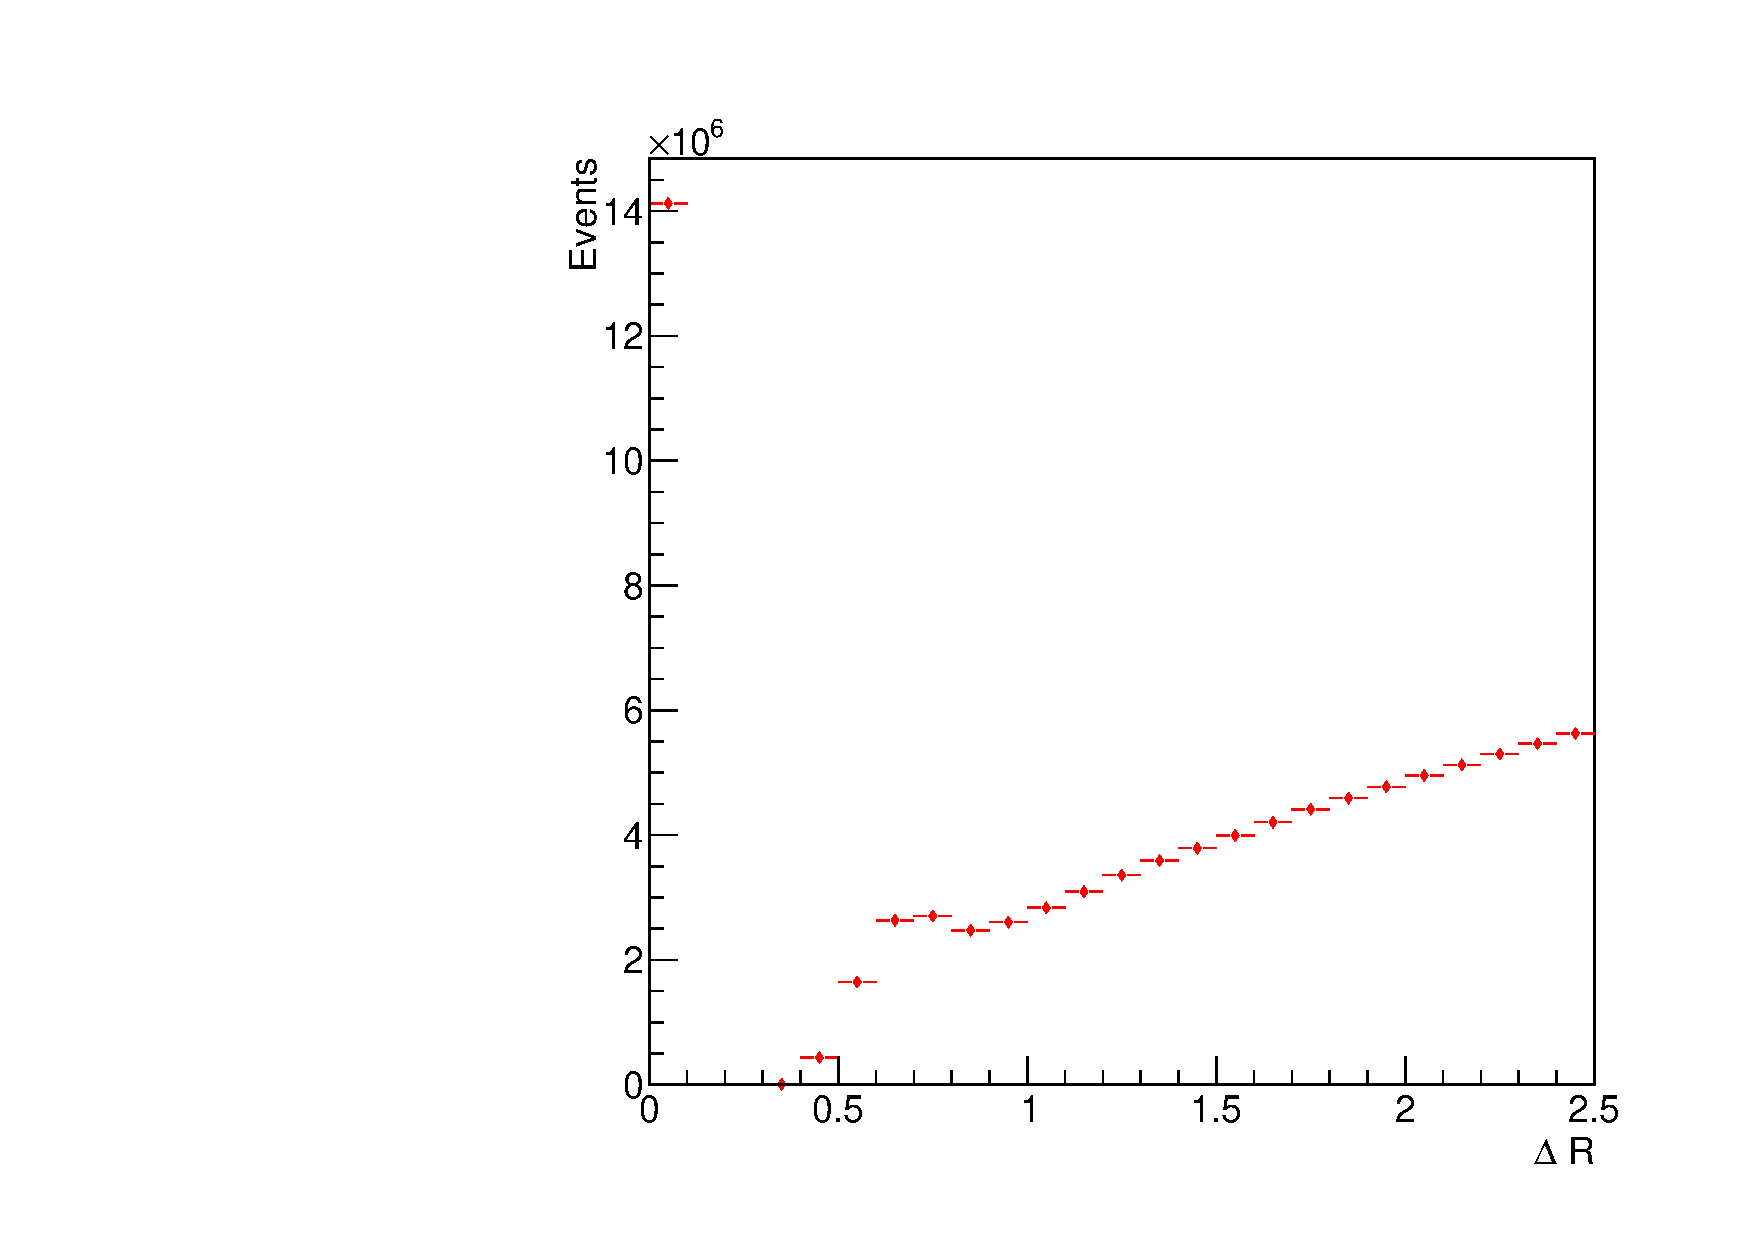
\includegraphics[width=0.5\linewidth]{deltaR}
	\caption[$\Delta R$ values for online/offline jet pairs in Monte-Carlo simulation]{Plot of $\Delta R$ values for all online/offline jet pairs taken from the Monte-Carlo simulations. The large spike at $\sim0$ accounts for matching jets, with the higher $\Delta R$ Values corresponding to differing jet pairs.}
	\label{f:deltaR}
\end{figure}
To compare the online and offline jets, the fractional
. difference in value for a variety of jet kinematic properties between the matched jets were evaluated. These values were calculated for jet feature $X$ using the ratio of the difference between the offline and online jet features to the offline jet feature

	\begin{equation}
	\frac{\Delta X}{X} = \frac{X_{Offline} - X_{Online}}{X_{Offline}}
	\end{equation}

	where $X_{Offline}$ is the value of the kinematic quantity for the offline jet and $X_{Online}$ is the same quantity for  the HLT jet. Of the kinematic jet quantities, jet \pt was the most significant value to study for a \VBFHBB\ analysis. In addition, the jet $\eta$ and $\phi$ values were compared to assess similarities between the topological distributions of the HLT and offline jets.

	These key kinematic quantities were studied for both the leading \bjet\ and the leading non-\bjet\, of an event given these jet types make up a \VBFHBB\ event. The jet objects were also divided into buckets of pseudo-rapidity described in Table \ref{tab:etabands} to examine any changes in behaviour in $\eta$, as any differences will significantly impact any assessment of the forward \VBFHBB\ jets.

	\begin{table}[h]
		\caption[Pseudorapidity bands of the object performance analysis]{Pseudorapidity bands.}
		\label{tab:etabands}
		\medskip
		\centering
		\begin{tabular}{cl}\toprule
			Jet Designation & $\eta$ Range \\\midrule
			Central & $0<|\eta|<1$ \\
			 & $1<|\eta|<2.4$  \\
			Forward & $2.4<|\eta|<4.9$ \\\bottomrule
		\end{tabular}\\[5pt]
	\end{table}

	The jets used to produce these plots were taken from all analysed Monte-Carlo events and all real data events where the \texttt{HLT\_j80\_bmv2c2070\_split\_\-j60\_bmv2c2085\_split\_j45\_320eta490} trigger was passed, but the additional \VBFHBB\, requirements mentioned in Section \ref{es:as} were not enforced. In addition, given the \pt requirements of the desired event are high, only jets with \pt$>45$GeV were considered for analysis.

\section{Leading \textit{b}-jets}
\label{OP:leadingb}

	The leading \pt offline $b$-jet was selected from an event, requiring the jet to pass the \textit{Tight} \btagging\ working point. This jet was matched to a corresponding online jet using $\Delta R$ matching, and the properties of each of these jets compared in both data and Monte-Carlo simulations. The \dptpt distribution for both the Monte-Carlo and data with respect to the \pt of the leading \bjet\ is shown in Figure \ref{fig:O:leadingbpt}.

		\begin{figure}[h]
			\centering
			\begin{minipage}[h]{0.48\linewidth}
				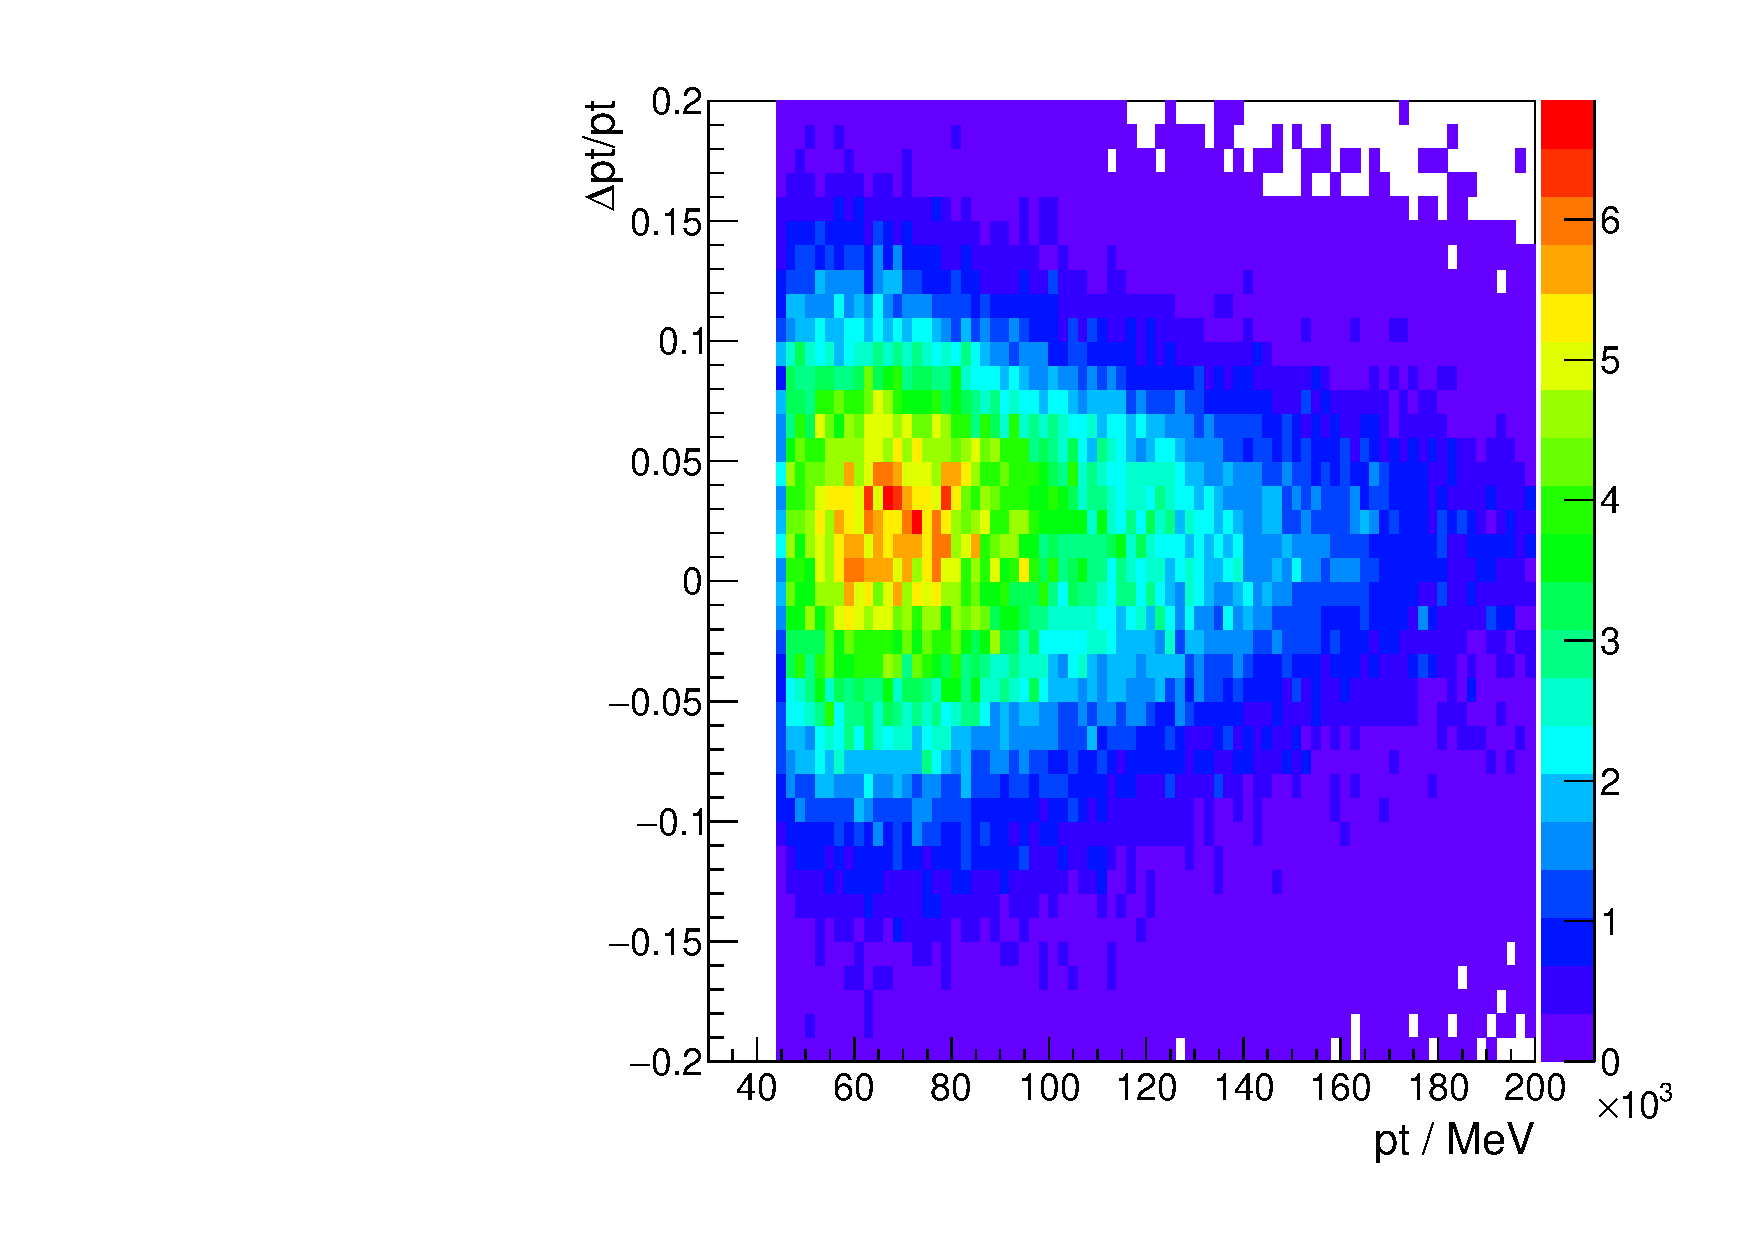
\includegraphics[width=1\linewidth]{ptRatio_Leading_BJet}

			\end{minipage}
			\quad
			\begin{minipage}[h]{0.48\linewidth}
				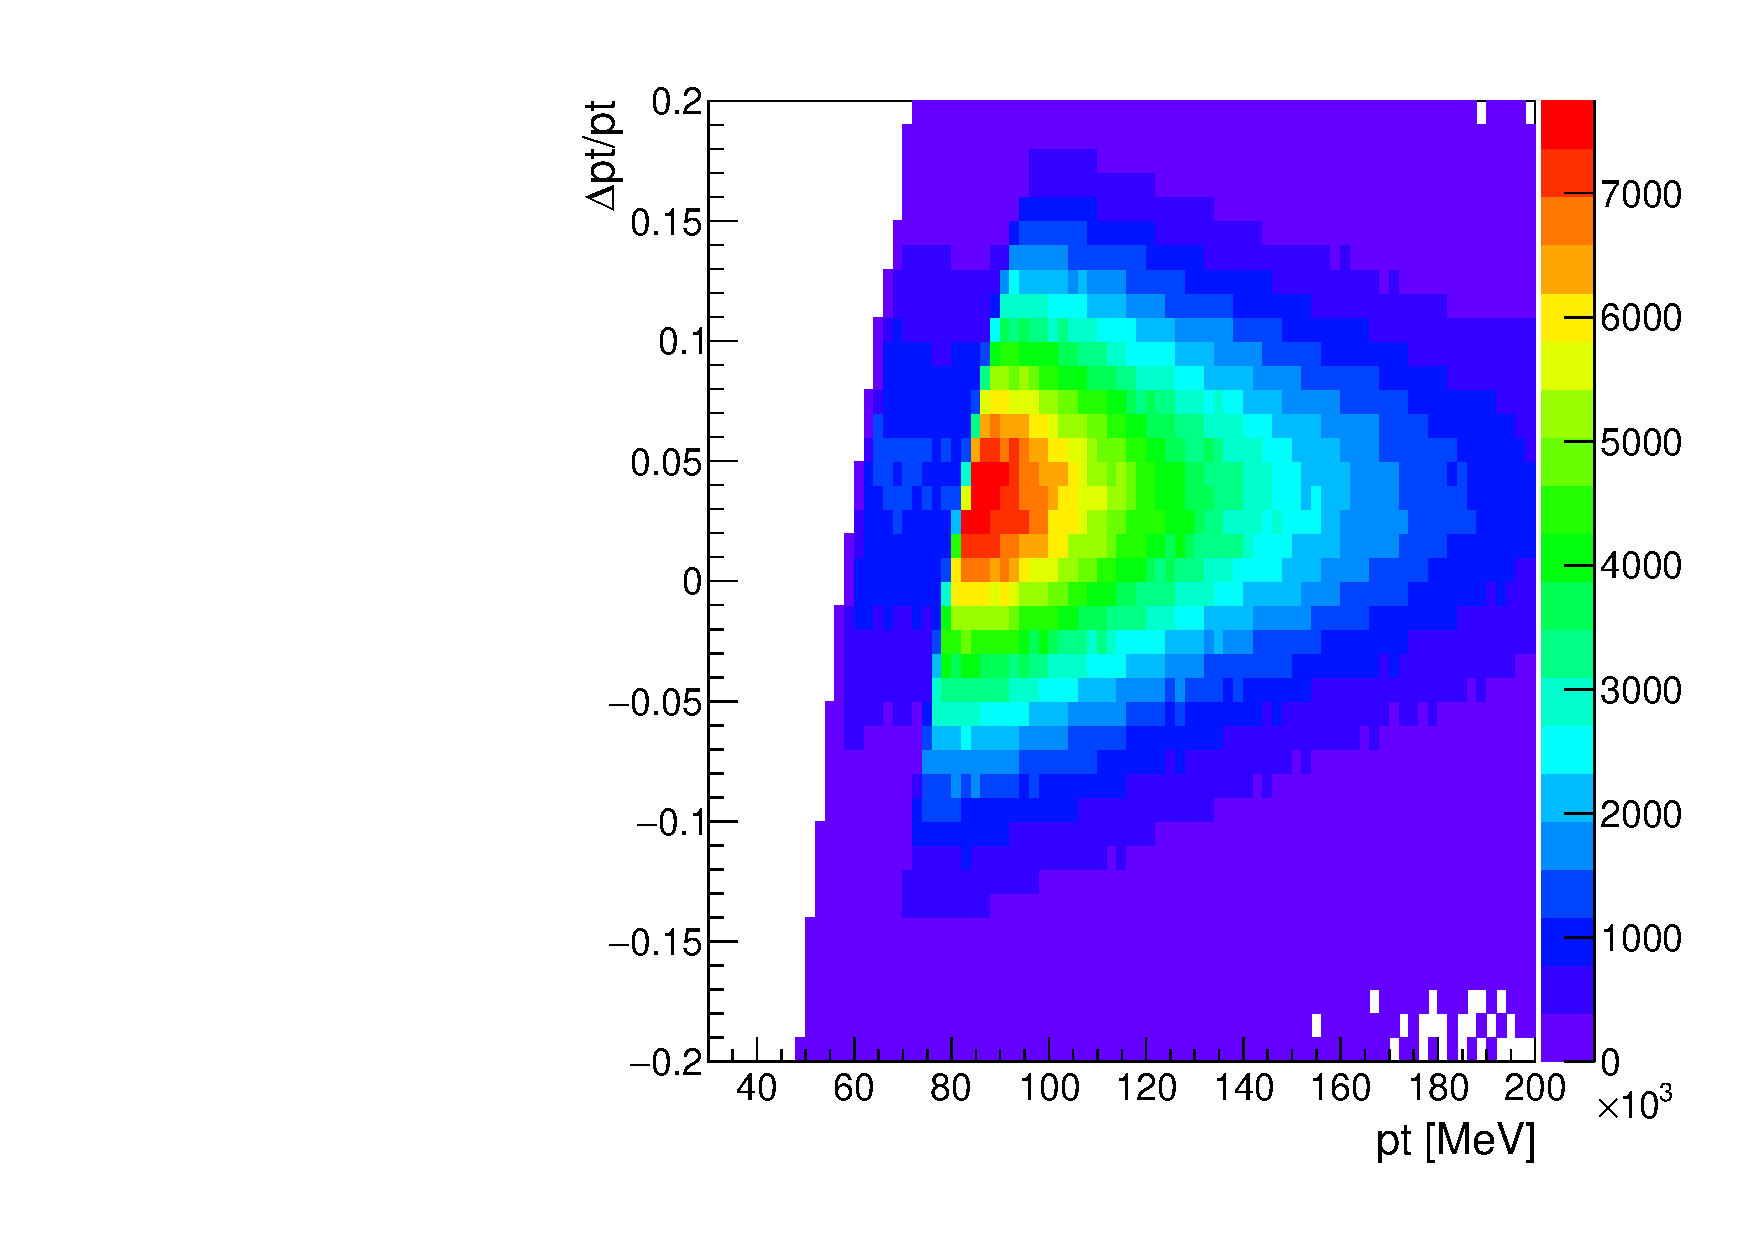
\includegraphics[width=1\linewidth]{Offline_2C_ptRatio_Leading_BJet}
			\end{minipage}
			\caption[\dptpt for the leading $b$-jet in data and Monte-Carlo simulations]{\dptpt for the leading \pt $b$-jet against \pt of the offline $b$-jet, plotted for Monte-Carlo simulation in the left panel and data in the right panel.}
			\label{fig:O:leadingbpt}
		\end{figure}

		\newpage
		The comparative performance of the online and offline jets in \pt is broadly similar for events in both data and Monte-Carlo simulations. The bulk of the results occur with a $0<$ \dptpt$<0.05$ and the two plots show a comparable distribution drop off, both showing a maximum \dptpt width of $-0.1 <$ \dptpt$<0.15$ and showing the \pt distribution reaching a maximum of $\sim80$GeV. The distinctive curved edge starting at \pt$\sim80$GeV present in the real data is the result of the trigger being applied to each event, which was not applied in the Monte-Carlo simulation. The trigger requires at least one jet with a \pt$>80$GeV which results in the small number of events below this cut value.

		The curve of the distribution shown in the right panel of Figure \ref{fig:O:leadingbpt} can be explained given \dptpt is predominantly positive. In the average case based on this, the \pt of the offline jet is higher than the online jet. As the trigger is evaluated on the online jet, only events with an online \pt$>80$GeV will be entered into this histogram. For an offline jet with \pt$=85$GeV to have \dptpt$=0.1$, the online jet would be less than the trigger \pt cut and as such will not enter into the plot shown in Figure \ref{fig:O:leadingbpt}. This exclusion of certain \dptpt values for certain offline \pt values follows from the demonstrated bias in \dptpt, and produces the curved edge of the distribution.

		The distribution of the \dptpt about zero can be shown in more detail by taking a slice across the distribution for a representative \pt value, which is shown in Figure \ref{fig:O:leadingbptslice} for leading \bjets\ with $89< $\pt$<91$GeV. The \dptpt values were also split into the $\eta$ bands from Table~\ref{tab:etabands}. For the leading \bjet, this is constrained to be within the region of the detector where \btag\, is available, so the forward band is excluded.

		\begin{figure}[h]
			\centering

			\begin{minipage}[h]{0.48\linewidth}
				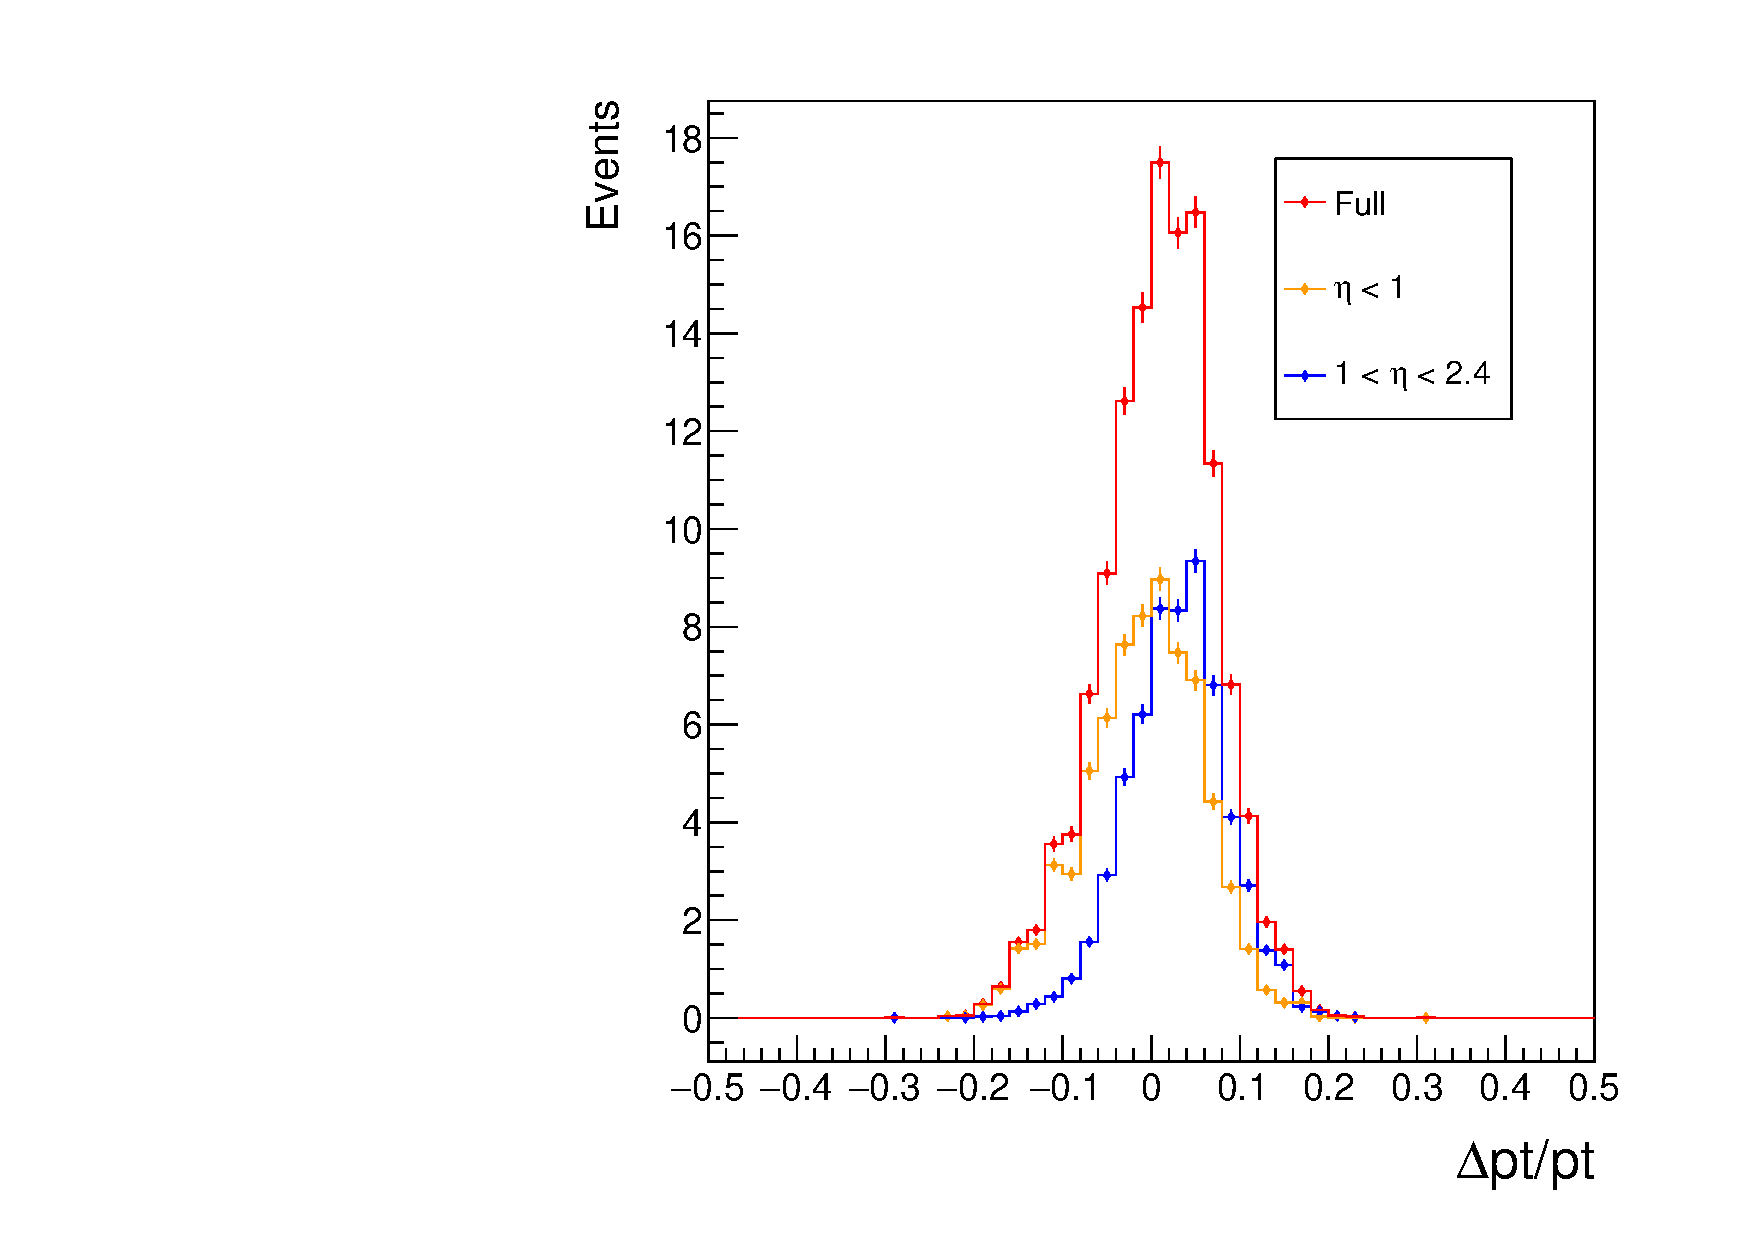
\includegraphics[width=1\linewidth]{Slices_ptRatio_Leading_BJet}
			\end{minipage}
			\quad
			\begin{minipage}[h]{0.48\linewidth}
				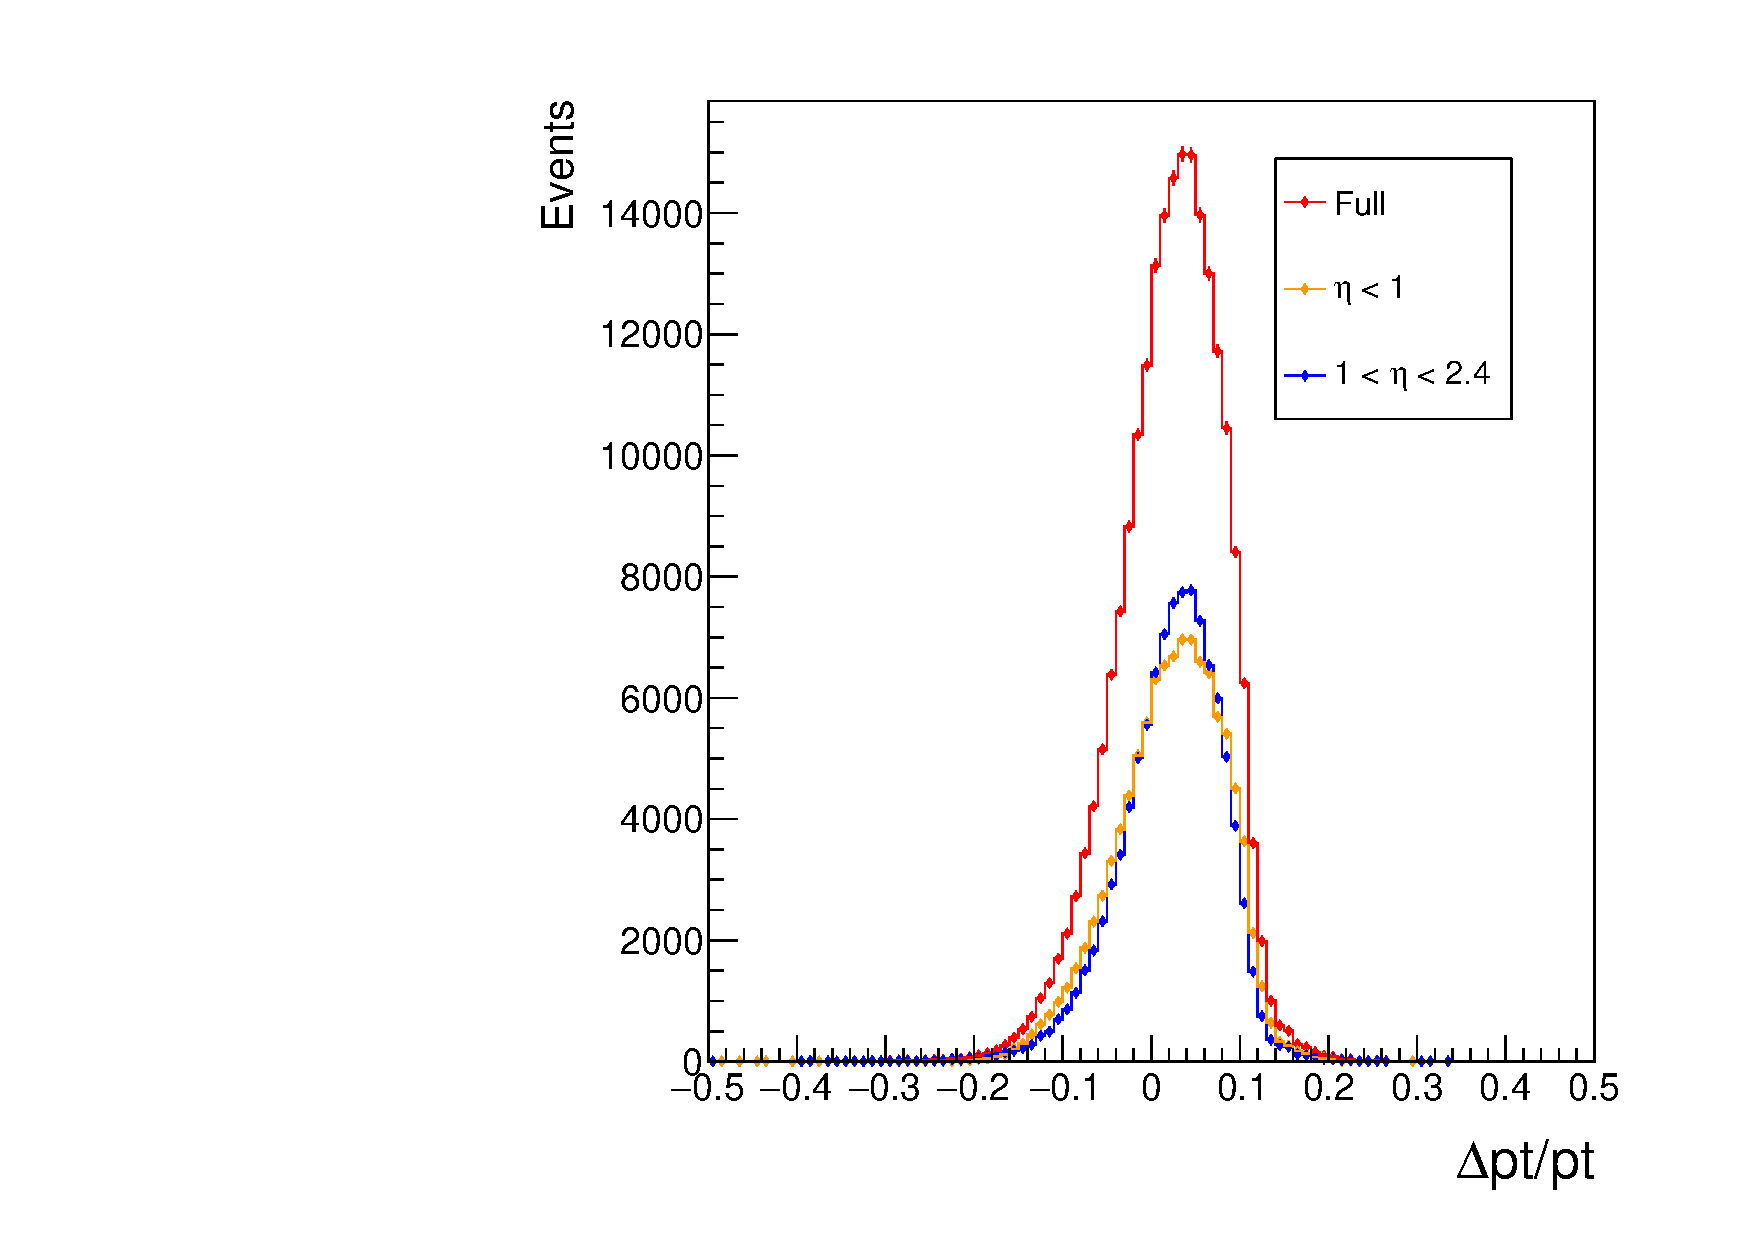
\includegraphics[width=1\linewidth]{Slices_Data_ptRatio_Leading_BJet}
			\end{minipage}
			\caption[\dptpt distribution for leading \bjets\ with $89<$\pt$<91$ in data and Monte-Carlo simulations]{\dptpt distribution for the leading \bjet\ with $89<$\pt$<91$ GeV. The distributions for all events and events split by $\eta$ region are shown. Monte-Carlo simulation is shown in the left panel and data in the right panel.}
			\label{fig:O:leadingbptslice}
		\end{figure}

		\newpage
		The results show similar profiles between the Monte-Carlo and Data events for $\frac{\Delta p_\text{T}}{p_\text{T}}$. Both plots show the median offline \pt values to be higher than the online, with a median shift of $4\%$ in data and $2\%$ in Monte-Carlo simulations. The performance between $\eta$ ranges was also consistent. The profiles broadly match the full shape of each other, but the Monte-Carlo plot in the left panel of Figure \ref{fig:O:leadingbptslice} showed a slight difference in \dptpt value as the central $\eta$ range peaked at approximately zero. The breadth of these distributions is quite large, with the data and Monte-Carlo simulations showing a $\frac{\Delta p_\text{T}}{p_\text{T}}$  distribution width of $\sim20\%$ about 0.

		This offset of the median \dptpt value shows that there is a difference in the jet energy calibration between the HLT and the offline reconstruction. The difference between the two is also shown by the offset peaks of the $\eta$ bands in Figure \ref{fig:O:leadingbptslice}, with the more central region performing better. Prior calibration studies of the ATLAS calorimeter have shown the energy readouts to be more consistent towards the central regions of the detector \cite{JES}. This could cause the inaccuracy of the trigger jets in the higher pseudorapidity regions, as offline jet reconstruction can make use of developed calibration tools to account for these differences. Using these standard tools, the energy scale calibration difference between the offline and online jets can be rectified for future analyses \cite{jetcalib, JES}.

		The \dxx comparisons can be carried out for the topological jet properties ($\eta$, $\phi$) to confirm the offline and online jets are positioned within the detector in a similar fashion. Plots of \dee against the pseudorapidity of the offline jet in the selected pair for data and Monte-Carlo simulation are shown in Figure \ref{fig:O:leadingbeta}, and comparable plots of \dphph against the offline $\phi$ are given in Figure \ref{fig:O:leadingbphi}.

		\begin{figure}[h]
			\centering
			\begin{minipage}[h]{0.48\linewidth}
				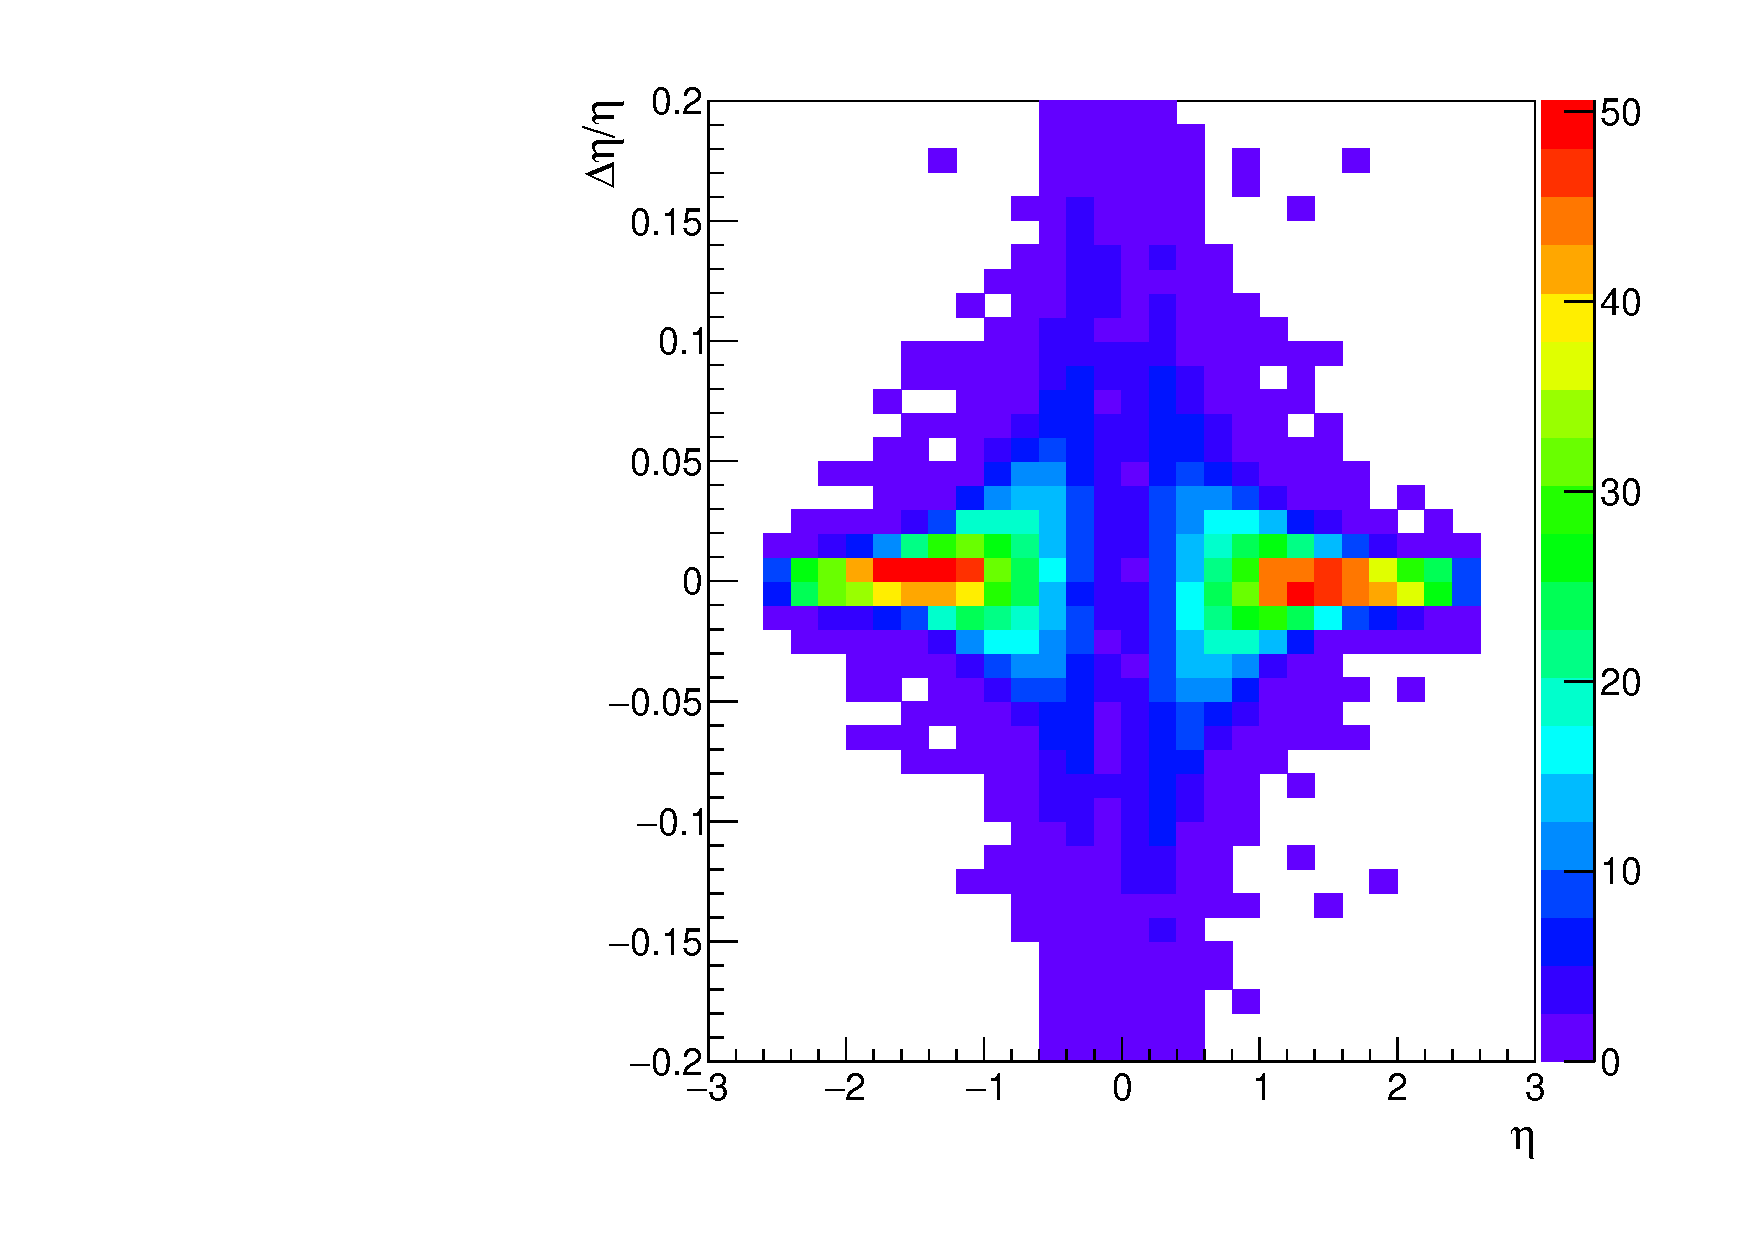
\includegraphics[width=1\linewidth]{etaRatio_Leading_BJet}

			\end{minipage}
			\quad
			\begin{minipage}[h]{0.48\linewidth}
				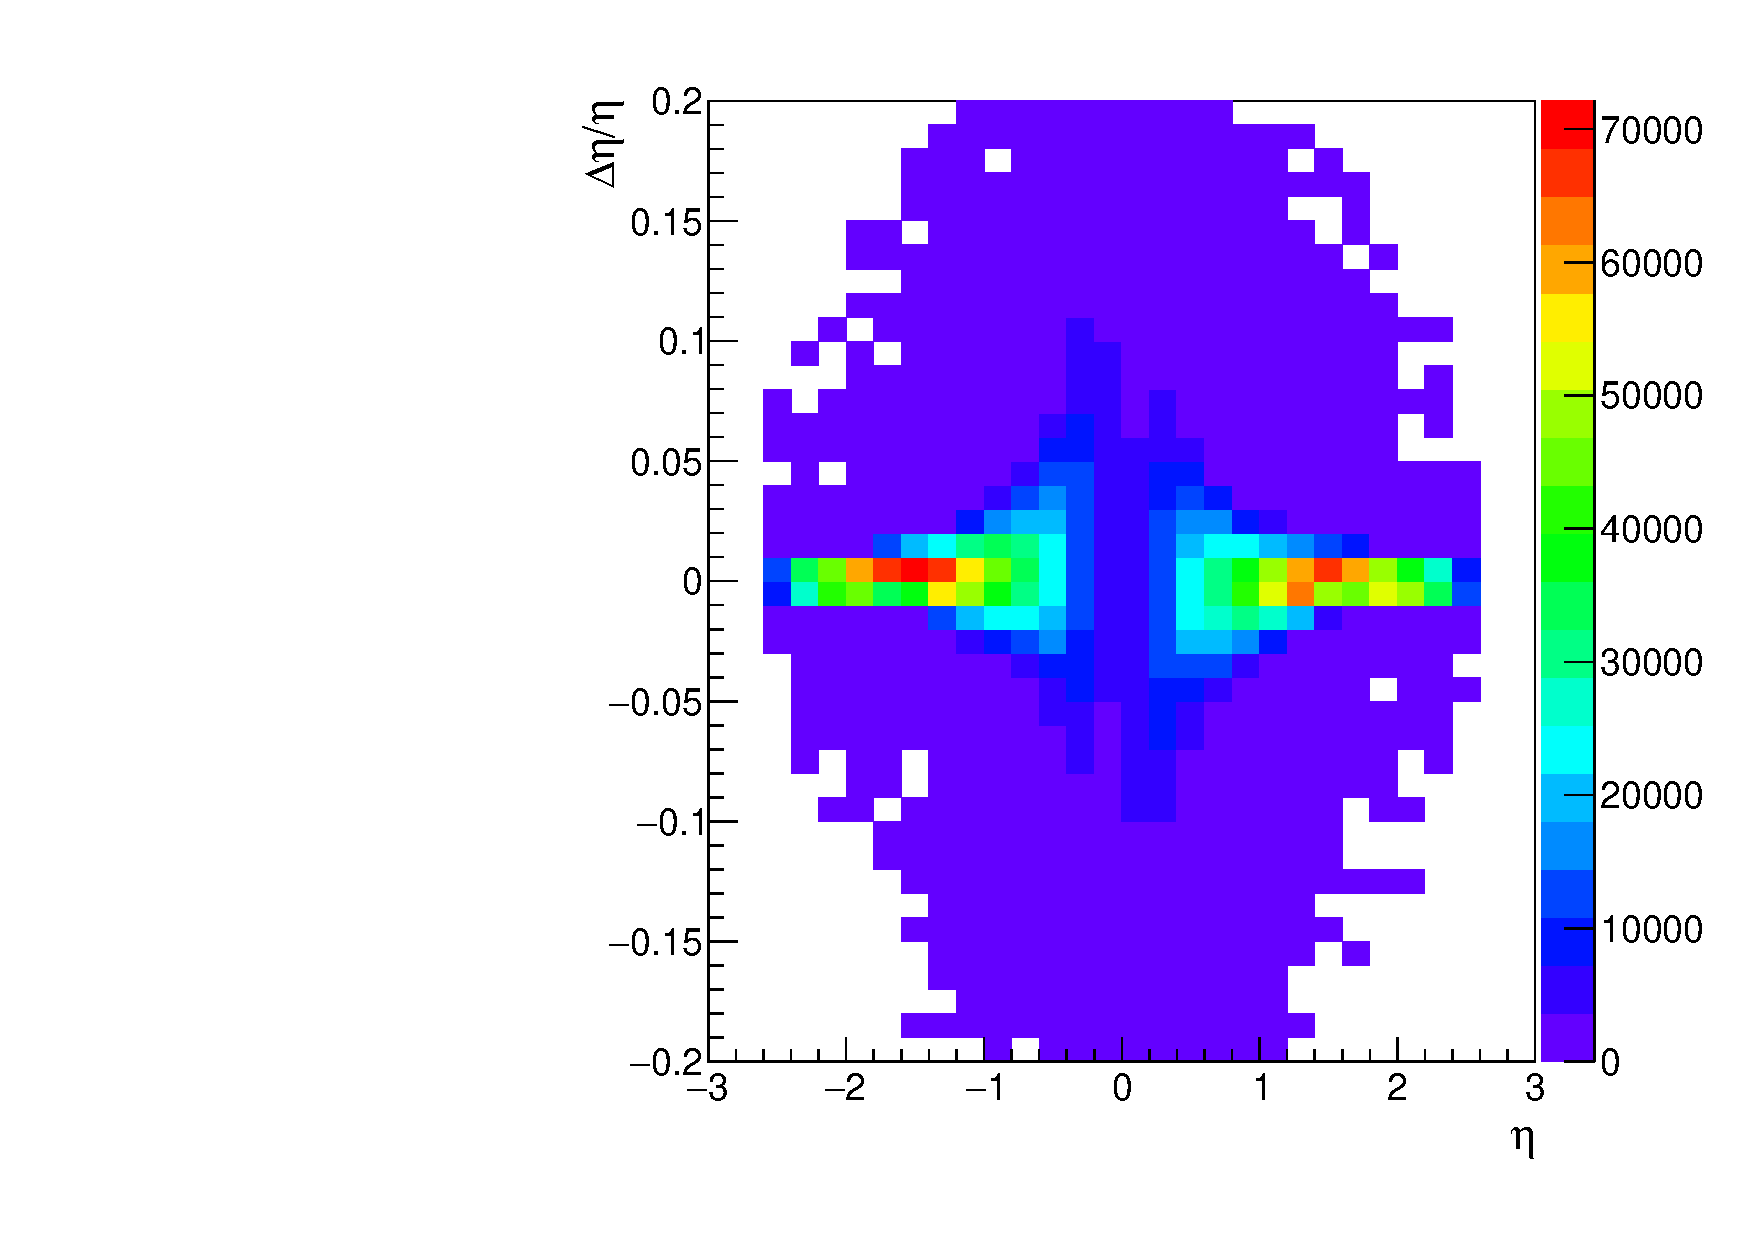
\includegraphics[width=1\linewidth]{Offline_2C_etaRatio_Leading_BJet}
			\end{minipage}
			\caption[\dee for the leading \bjet\ in data and Monte-Carlo simulations]{\dee for the leading \bjet, for Monte-Carlo simulation in the left panel and data in the right panel.}
			\label{fig:O:leadingbeta}
		\end{figure}

		\begin{figure}[h]
			\centering
			\begin{minipage}[h]{0.48\linewidth}
				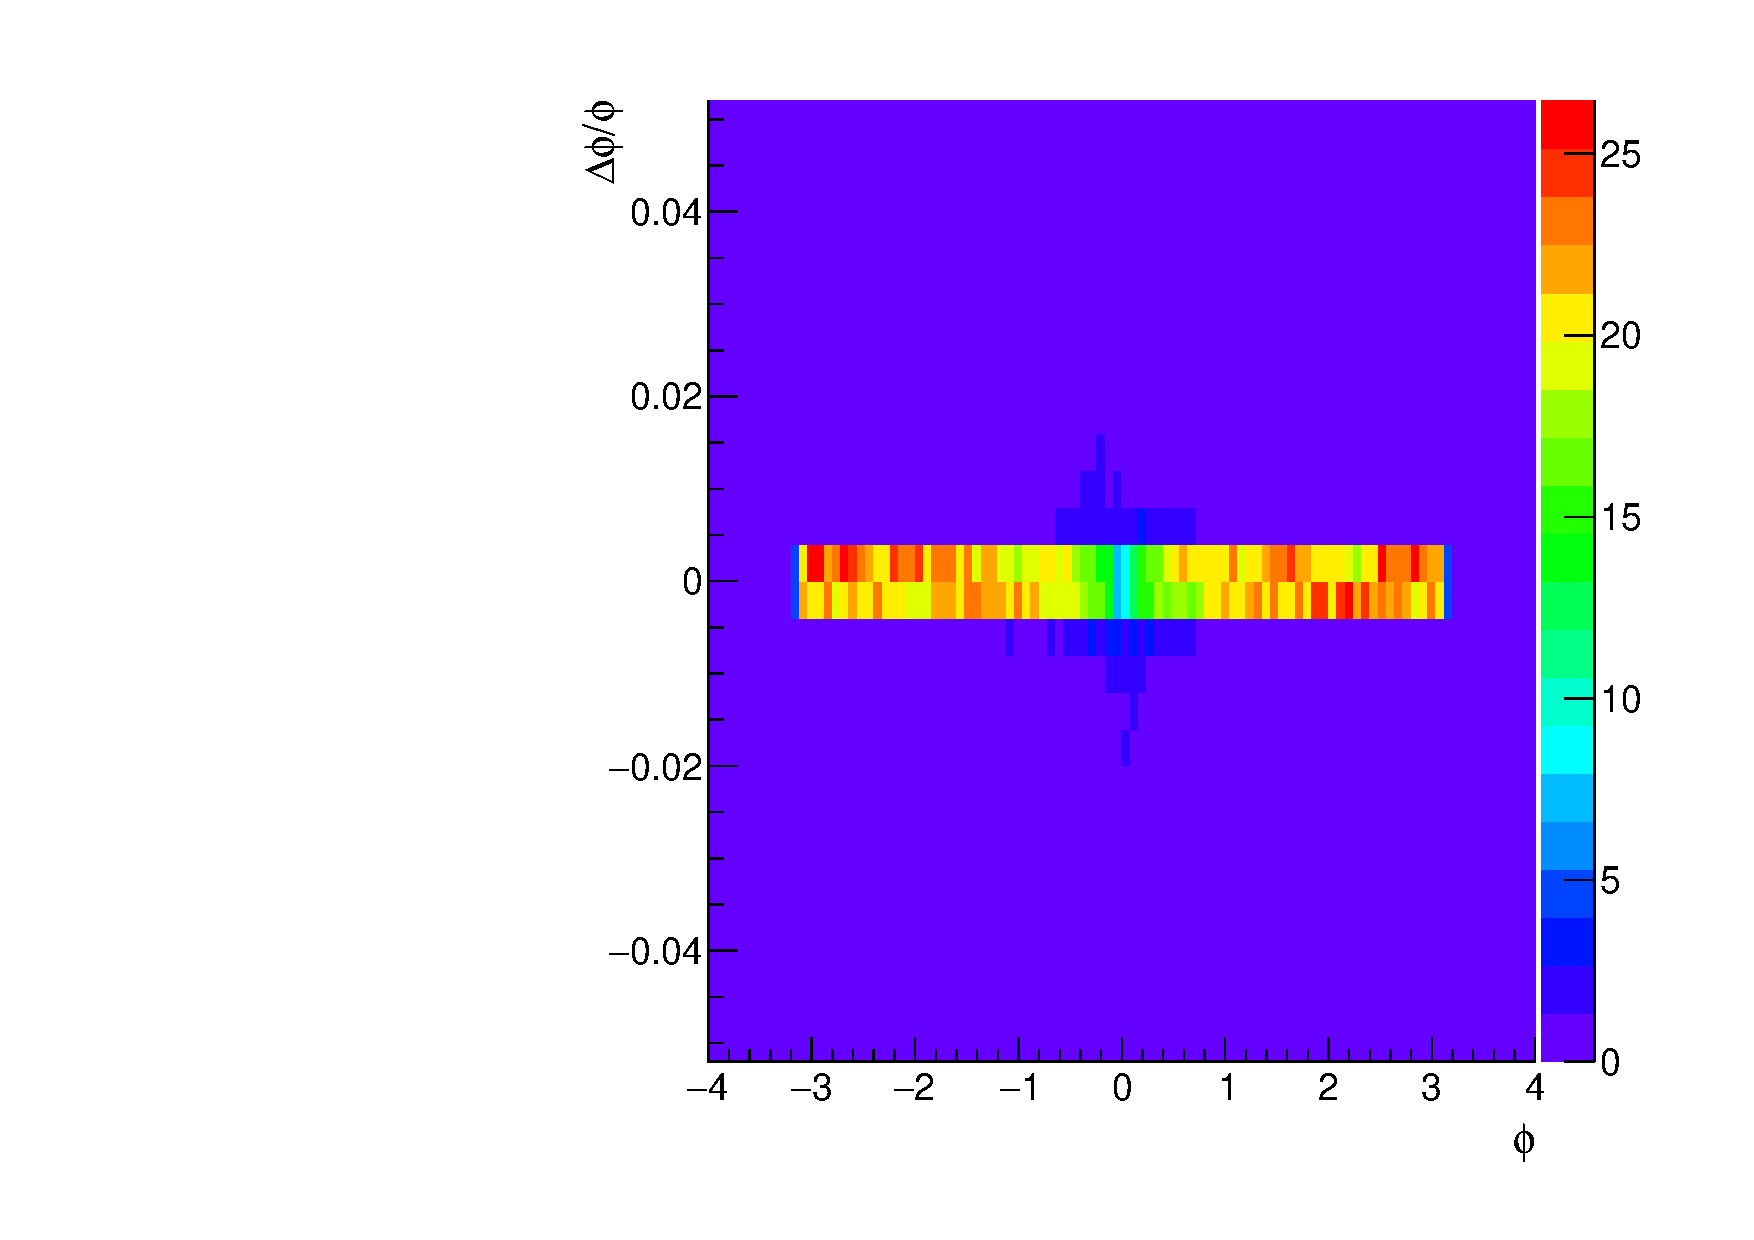
\includegraphics[width=1\linewidth]{phiRatio_Leading_BJet}

			\end{minipage}
			\quad
			\begin{minipage}[h]{0.48\linewidth}
				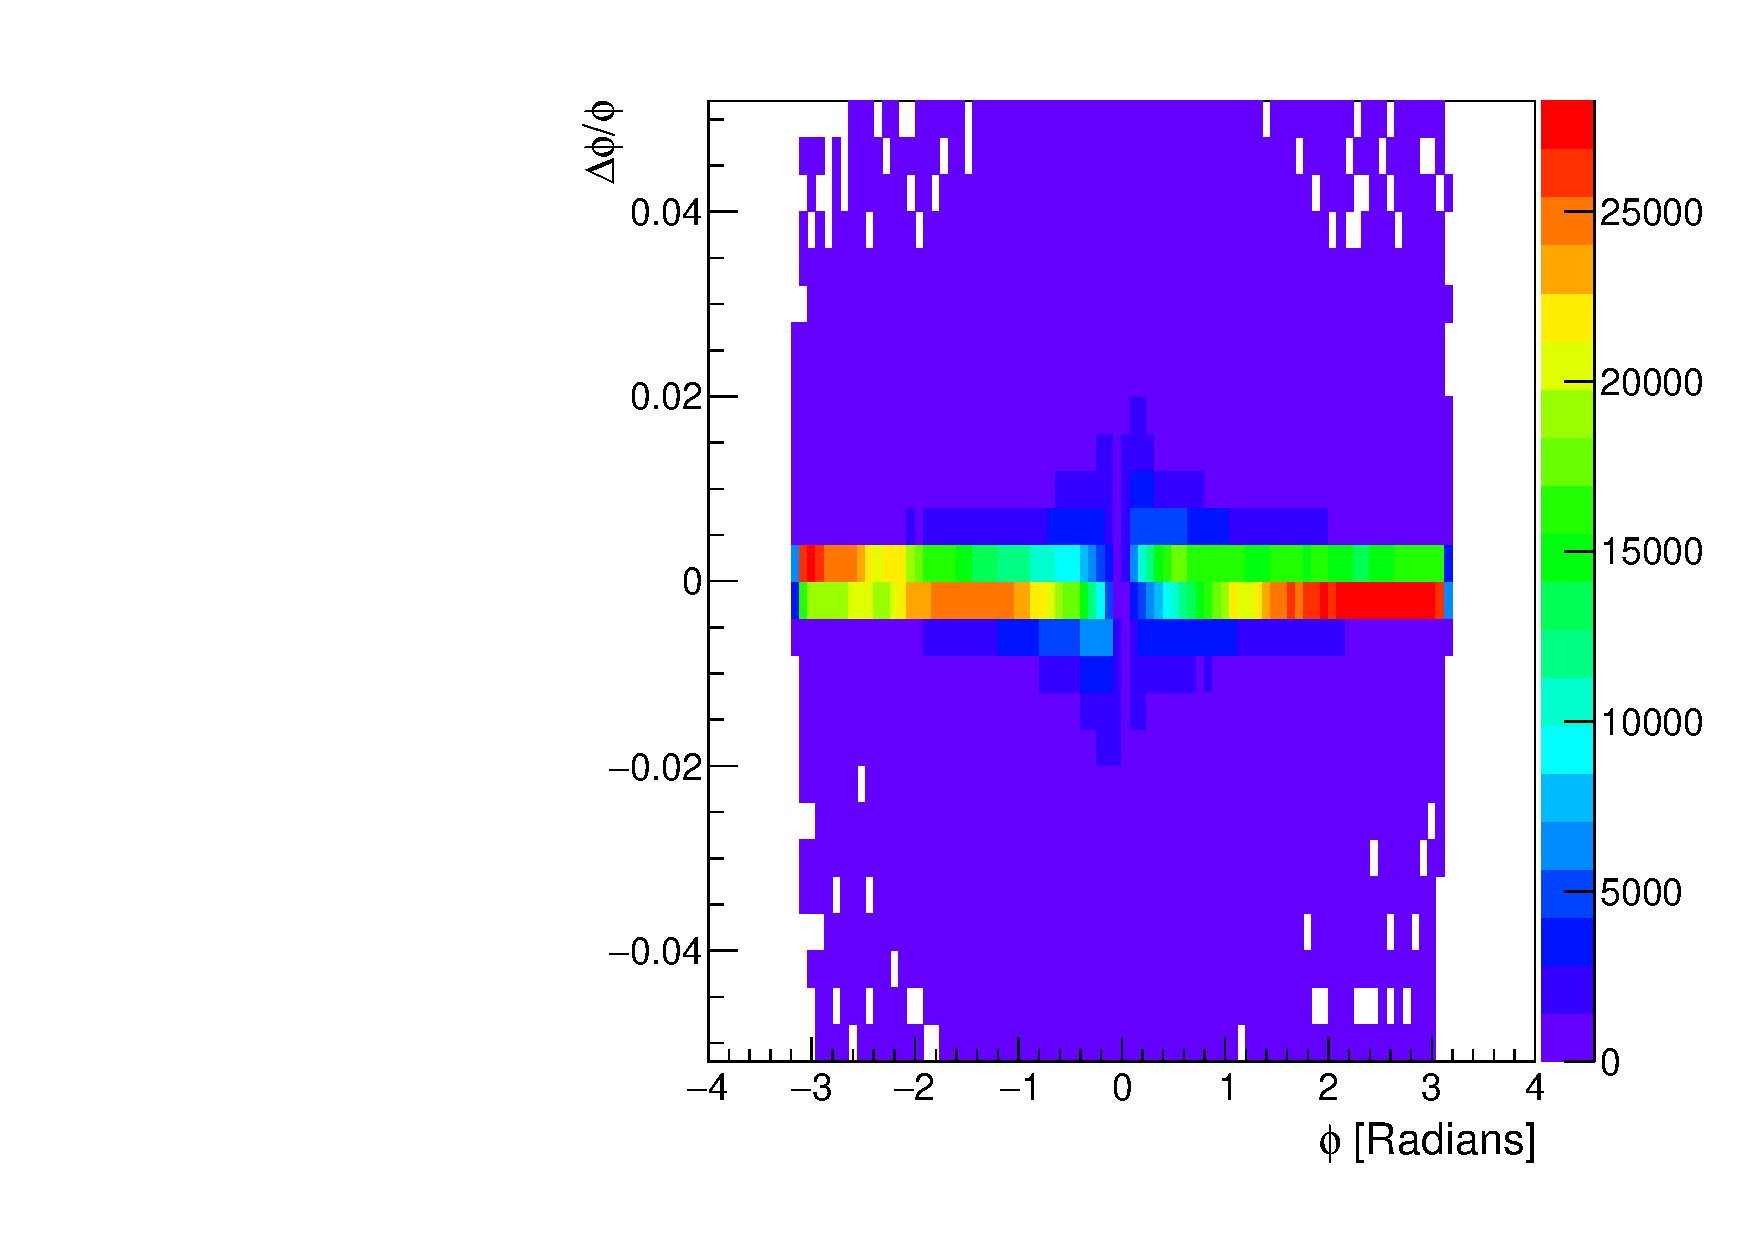
\includegraphics[width=1\linewidth]{Offline_2C_phiRatio_Leading_BJet}
			\end{minipage}
			\caption[\dphph for the leading \bjet\ in data and Monte-Carlo simulations]{\dphph for the leading \bjet, for Monte-Carlo simulation in the left panel and data in the right panel.}
			\label{fig:O:leadingbphi}
		\end{figure}

		\newpage
		The data and Monte-Carlo distributions for these values are extremely similar to each other, and also show very close agreement between the values for offline and online jet objects. For both \dee and \dphph the median value is approximately zero and the width of the distribution is less than $1\%$ of the value. These results show the ($\eta, \phi$) positions of the online and offline jet objects are comparable to each other.


\newpage
\section{Leading Non \textit{b}-jets}
	\label{OP:leadingnonb}

	For \VBFHBB\,, a pair of high \pt forward jets is the other significant feature, so the offline/online performance in the leading non-\bjet\ was studied. Identically to the analysis of the leading \bjet\ in Section \ref{OP:leadingb}, the \pt, $\eta$ and $\phi$ values of a matched offline/online jet pair were studied by calculating \dxx values and plotting against the offline kinematic quantity. The results could be split into the $\eta$ bands from Table \ref{tab:etabands}, with the forward pseudorapidity band available for analysis as \btag\ was not required. Plots of \dptpt for the leading non-\bjet\ are shown in Figure \ref{fig:O:leadingnonbpt}.

	\begin{figure}[h]
		\centering
		\begin{minipage}[h]{0.48\linewidth}
			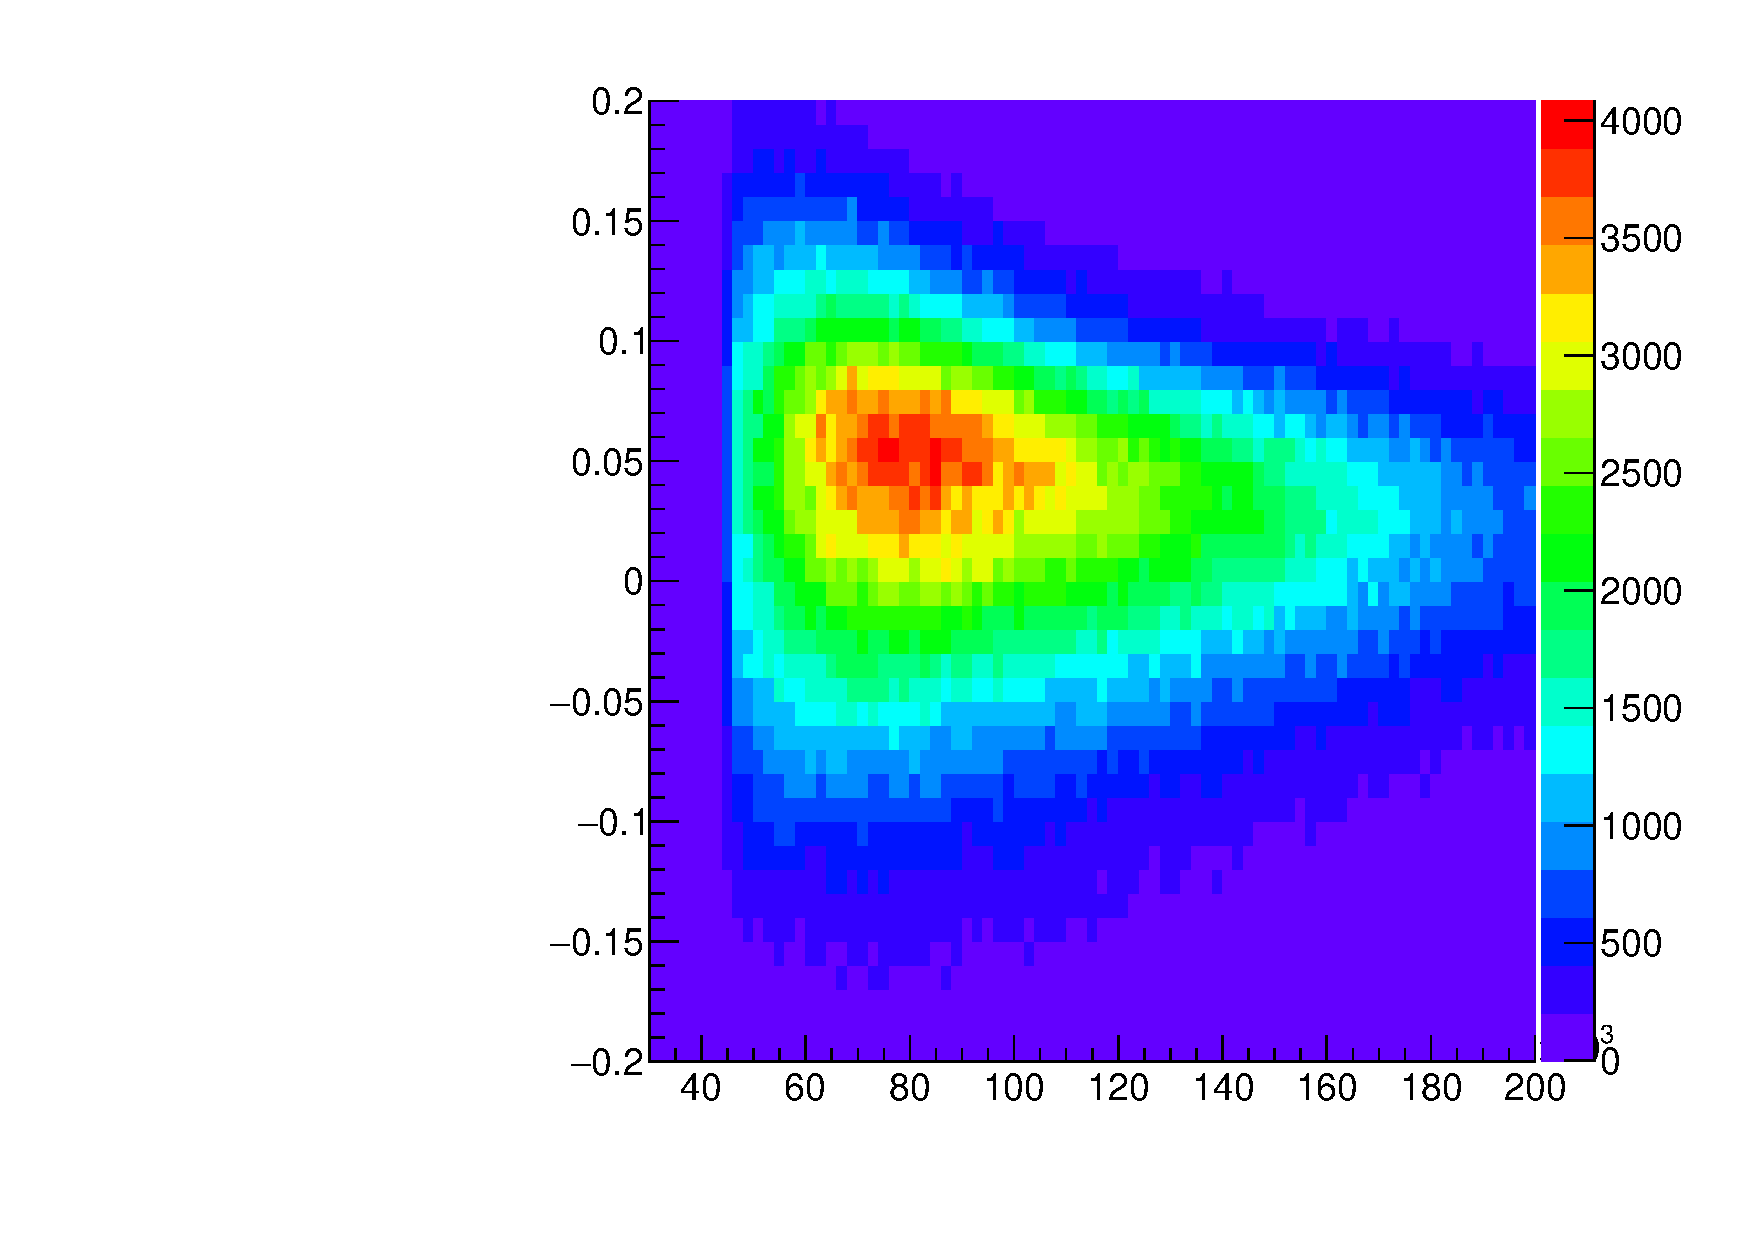
\includegraphics[width=1\linewidth]{ptRatio_Leading_Non_BJet}

		\end{minipage}
		\quad
		\begin{minipage}[h]{0.48\linewidth}
			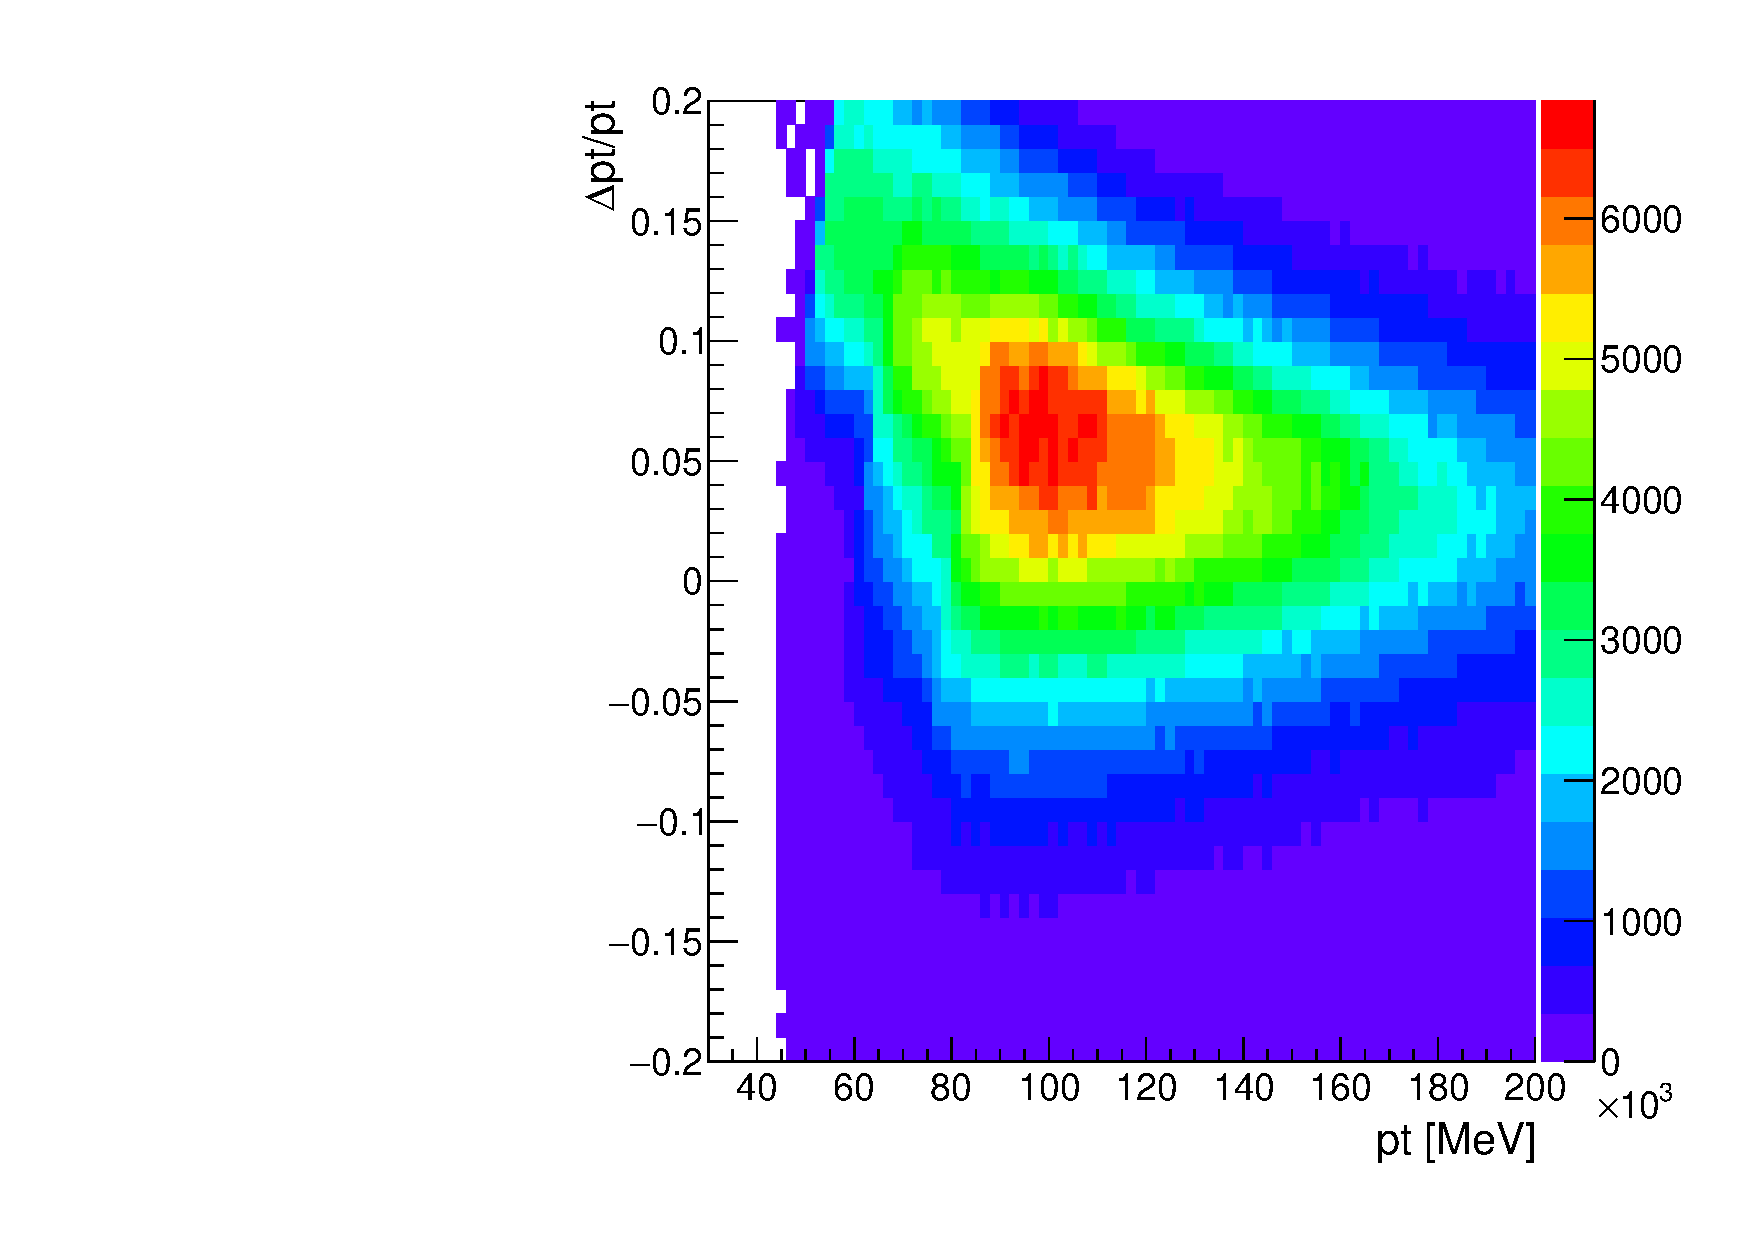
\includegraphics[width=1\linewidth]{Offline_2C_ptRatio_Leading_Non_BJet}
		\end{minipage}
		\caption[\dptpt for the leading \pt non-$b$-jet in data and Monte-Carlo simulations]{\dptpt for the leading \pt non-$b$-jet against \pt of the offline jet, plotted for Monte-Carlo simulation in the left panel and real data in the right.}
		\label{fig:O:leadingnonbpt}
	\end{figure}

	The leading non-\bjet\ distributions show similar results to the leading \bjet\ distributions in Figure \ref{fig:O:leadingbpt}. The peak of the distribution between $0<$ \dptpt$<0.1$ shows there is agreement between the \pt of the offline and the online non-\bjet. The overall shape of the distribution shows some differences between the Monte-Carlo simulation and data however. The distributions are similarly structured, with a \dptpt width between $-0.1$ and $0.15$ and the \pt offline distribution reaching a maximum value of $\sim180$GeV. However, there is a distinct cluster of results shown only in the right panel of Figure \ref{fig:O:leadingnonbpt} of low \pt offline jets with \dptpt$>0.1$. There is also a suggestion of a curving edge to the distribution for the data, in an opposite direction to that shown for the leading \bjet\ in Figure \ref{fig:O:leadingbpt}. In addition, the peak of the data is slightly higher in \pt ($\sim80$-$120$GeV) than in the Monte-Carlo simulations ($\sim60$-$110$GeV).

	\newpage
	The slight upward shift in \pt can be explained by the \pt requirements of the trigger applied only to the data. Requiring the jet components to exceed high \pt cuts will bias the results to events containing high \pt jets, accounting for the upward \pt shift of the data events in the right panel of Figure \ref{fig:O:leadingnonbpt} relative to the left.

	As for the leading \bjet, slices can be taken of the \dptpt distribution to show the spread of values more clearly. Plots of \dptpt values for leading non-\bjets\ with $89<$ \pt$<91$GeV are shown for Monte-Carlo simulation and data in Figure \ref{fig:O:leadingnonbptslice}, and results have been split into the pseudorapidity bands from Table \ref{tab:etabands}.

	\begin{figure}[h]
		\centering

		\begin{minipage}[h]{0.48\linewidth}
			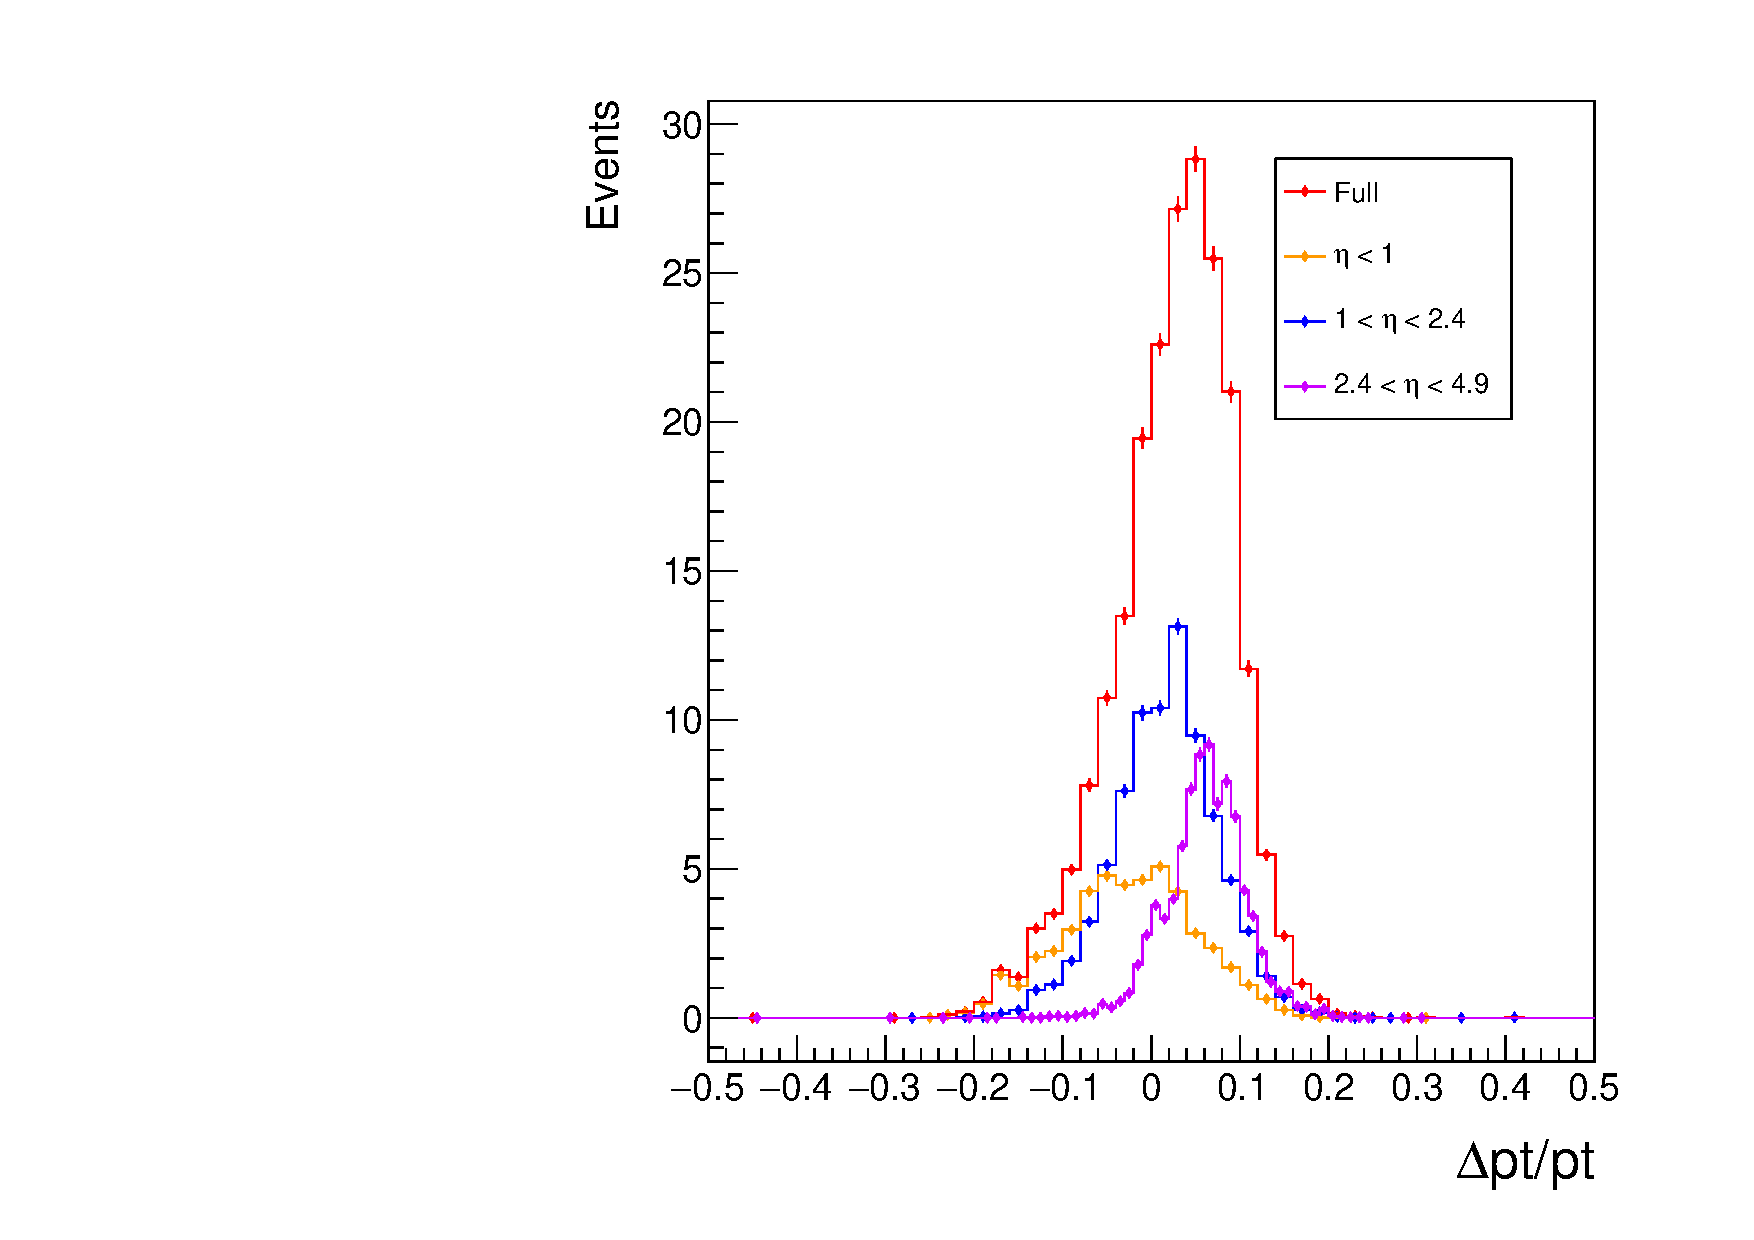
\includegraphics[width=1\linewidth]{Slices_ptRatio_Leading_Non_BJet}
		\end{minipage}
		\quad
		\begin{minipage}[h]{0.48\linewidth}
			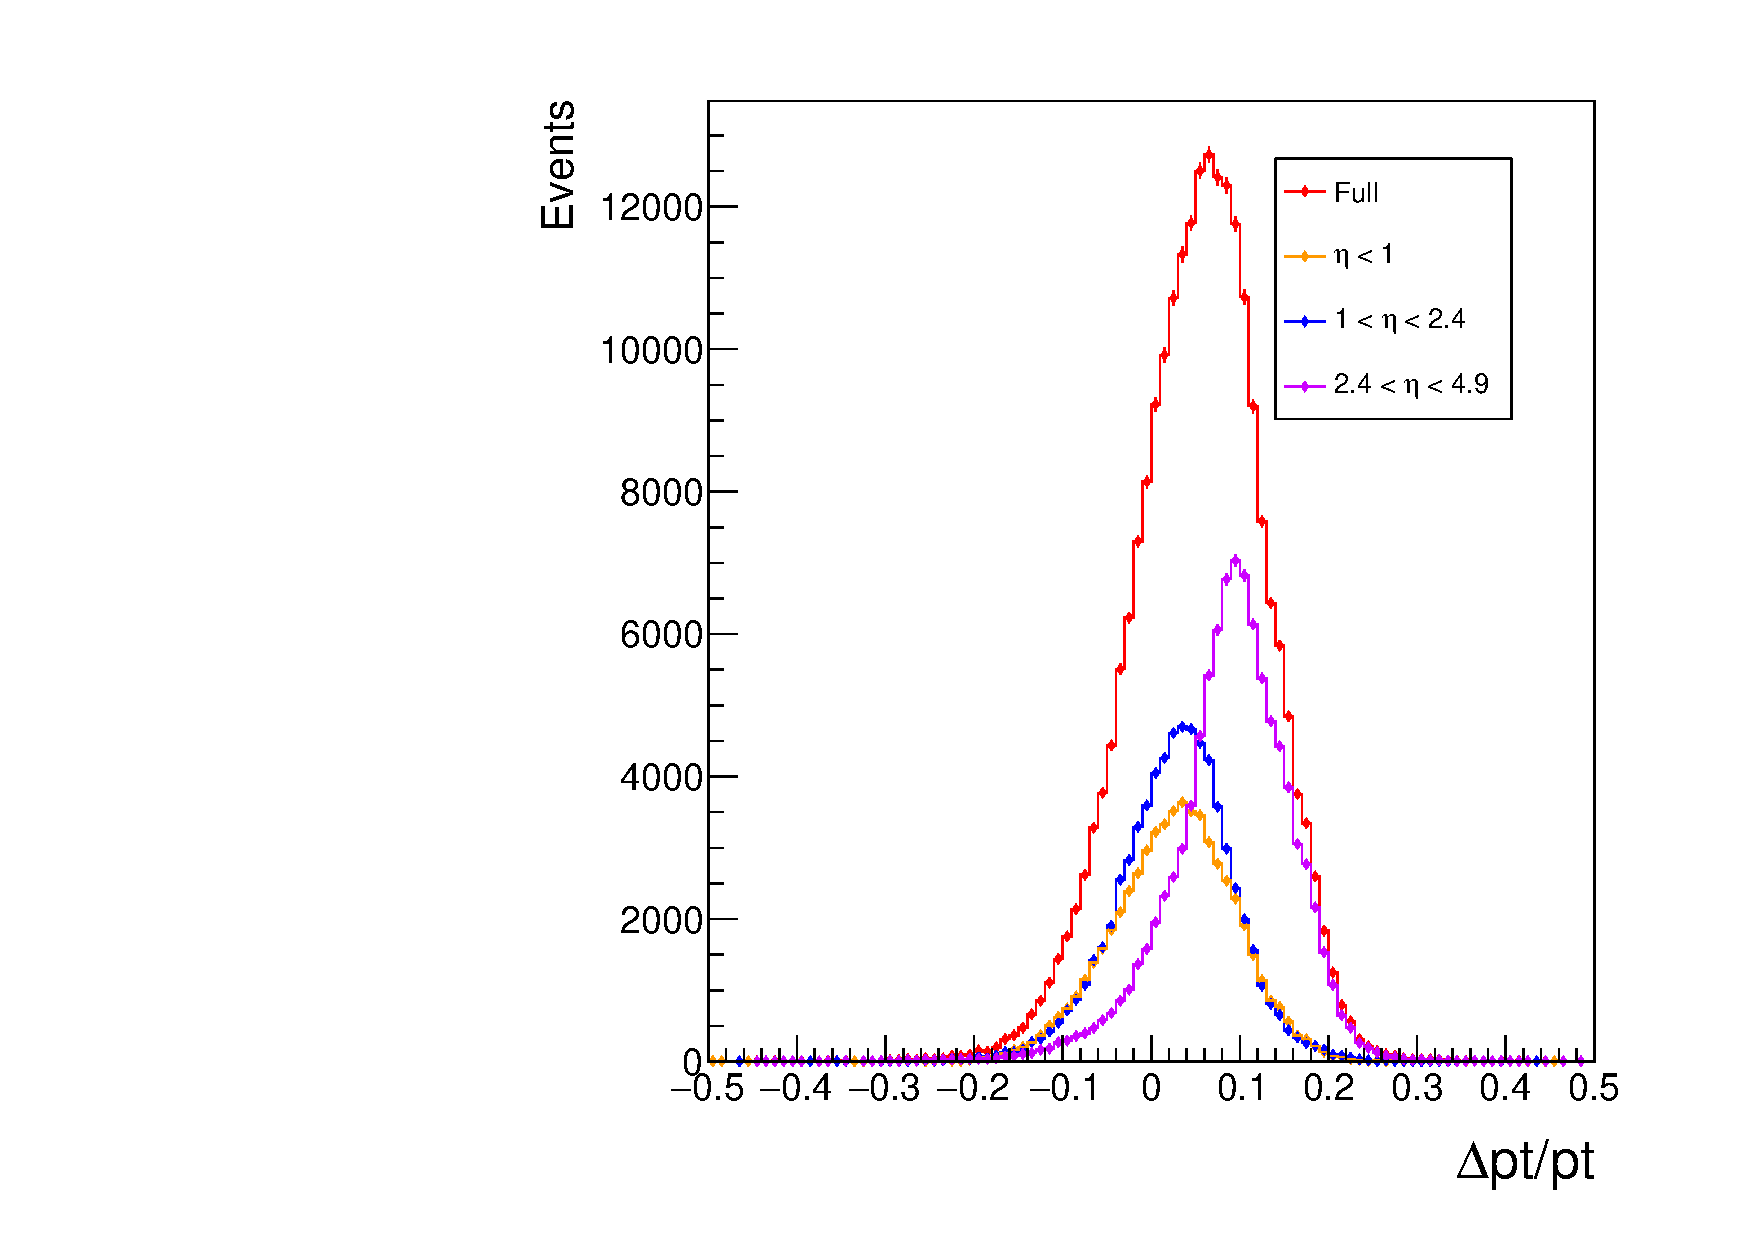
\includegraphics[width=1\linewidth]{Slices_Data_ptRatio_Leading_Non_BJet}
		\end{minipage}
		\caption[\dptpt distribution for leading non-\bjets\ with $89<$\pt$<91$ in data and Monte-Carlo simulations]{\dptpt distribution for the leading non-\bjet, with $89<$\pt$<91$ GeV plotted for Monte-Carlo simulation in the left panel and data in the right panel. The distributions for all events and events split by $\eta$ region are shown.}
		\label{fig:O:leadingnonbptslice}
	\end{figure}

	Both Monte-Carlo simulations and data show the median value for offline jet \pt to be higher than the online jet by $4\%$ and $6\%$ respectively. The overall distribution shape is similar between the simulated and real events for the full set of results, but the distributions for the $\eta$ bands differ between the Monte-Carlo simulations and the data.

	The Monte-Carlo results for the central $\eta$ band show a dip in \pt at the centre of the distribution and are shifted in \dptpt towards the negative. Both the data and Monte-Carlo show that the \dptpt value is much closer to zero for the two central $\eta$ bands than the forward band, which peaks significantly higher than the median \dptpt value. The offset of the forward $\eta$ band from the median is much worse for the data in the right panel of Figure \ref{fig:O:leadingnonbptslice}. In addition, the relative proportions of the three $\eta$ bands differ. In Monte-Carlo results most jets fell in the middle $1<|\eta|<2.4$ region, while the data showed significantly more forward jets.

	\newpage
	The relatively increased proportion of forward jets is likely a consequence of the \texttt{HLT\_j80\_\-bmv2c2070\_split\_\-j60\_bmv2c2085\_split\_j45\_320eta490} trigger being applied to the data. As the data events are required to have a forward jet to be stored in the histogram, this will bias the results to contain a greater proportion of forward jets, leading to the larger peak.

	The \dptpt results for the leading non-\bjet\, as for the leading \bjet\, show a difference in energy calibration between the HLT jet objects and the reconstructed offline objects. This difference in calibration can be corrected using standard jet calibration tools to bring the \pt values into closer agreement with one another \cite{JES, jetcalib}.

	\begin{figure}[h]
		\centering
		\begin{minipage}[h]{0.47\linewidth}
			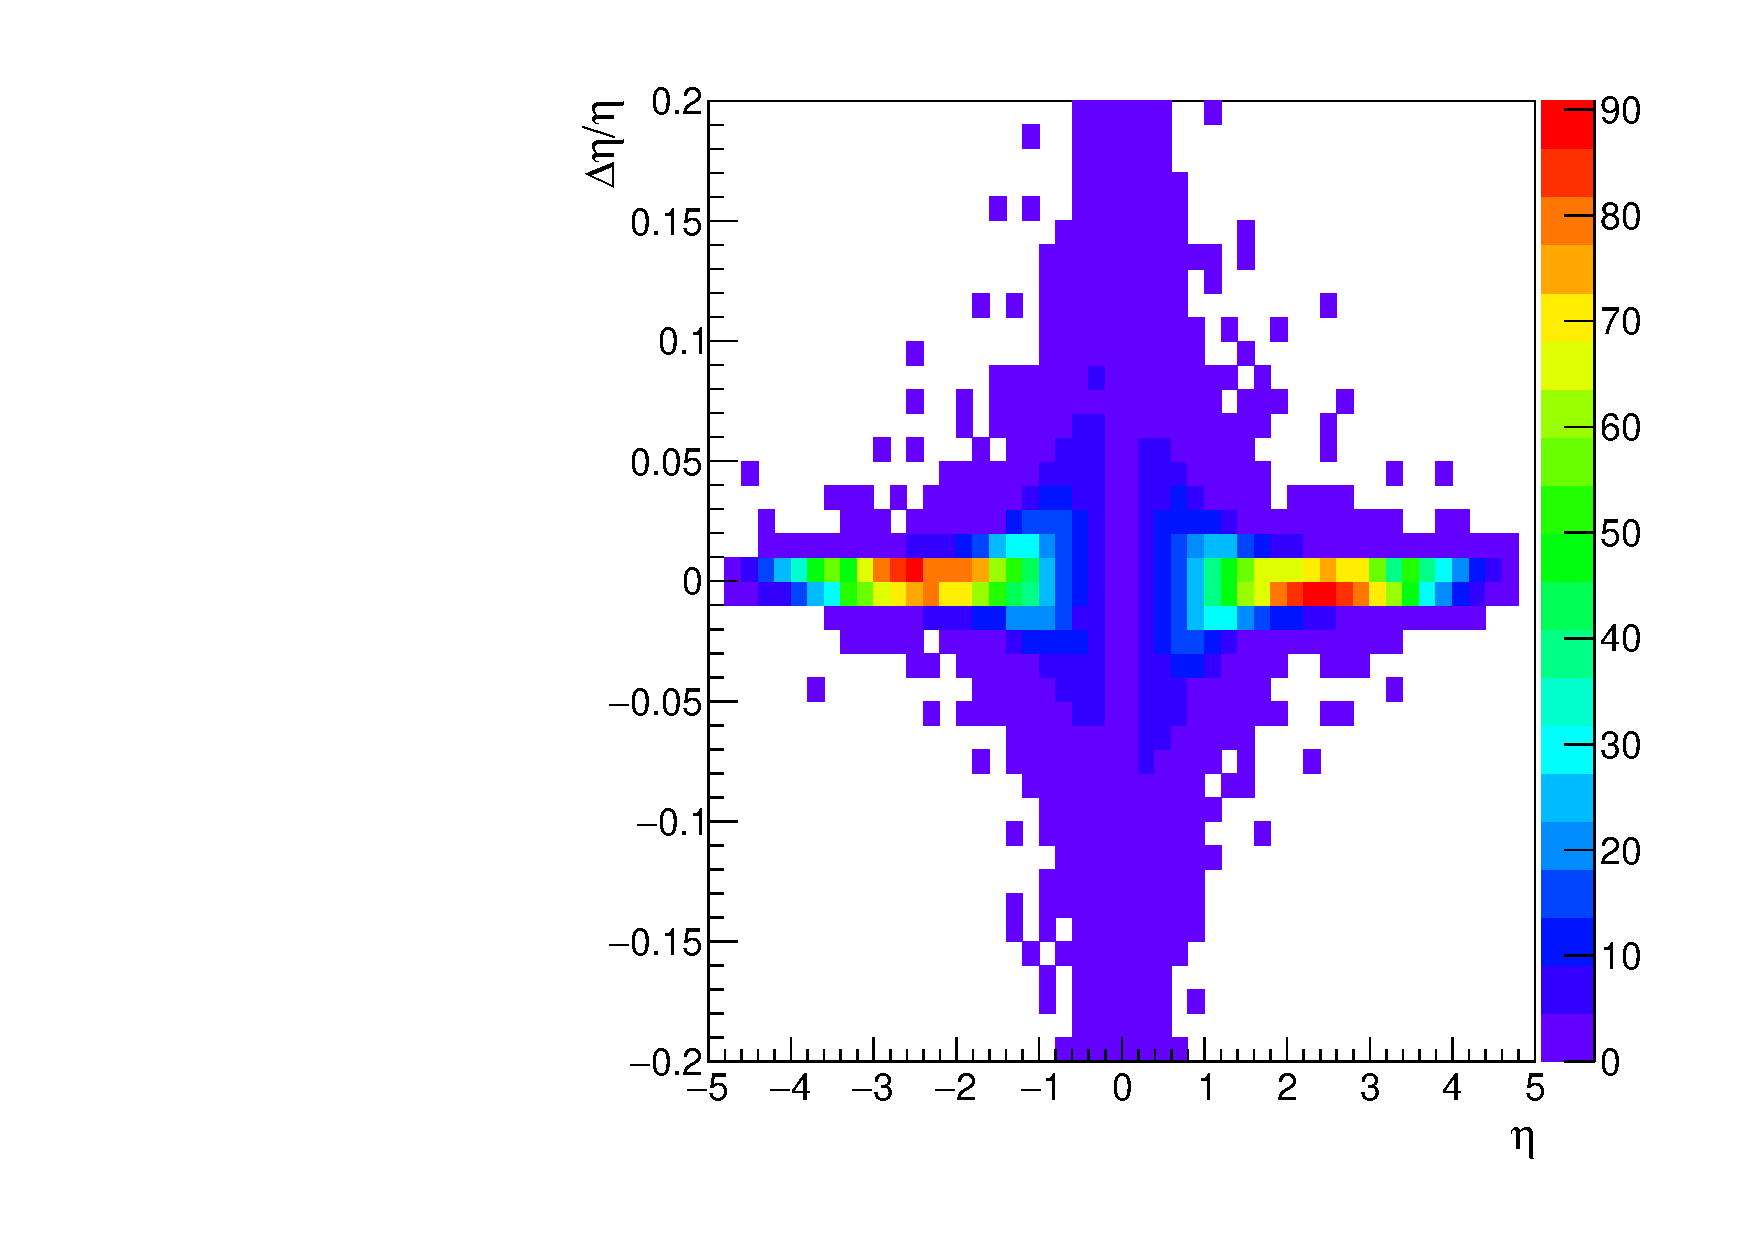
\includegraphics[width=1\linewidth]{etaRatio_Leading_Non_BJet}

		\end{minipage}
		\begin{minipage}[h]{0.47\linewidth}
			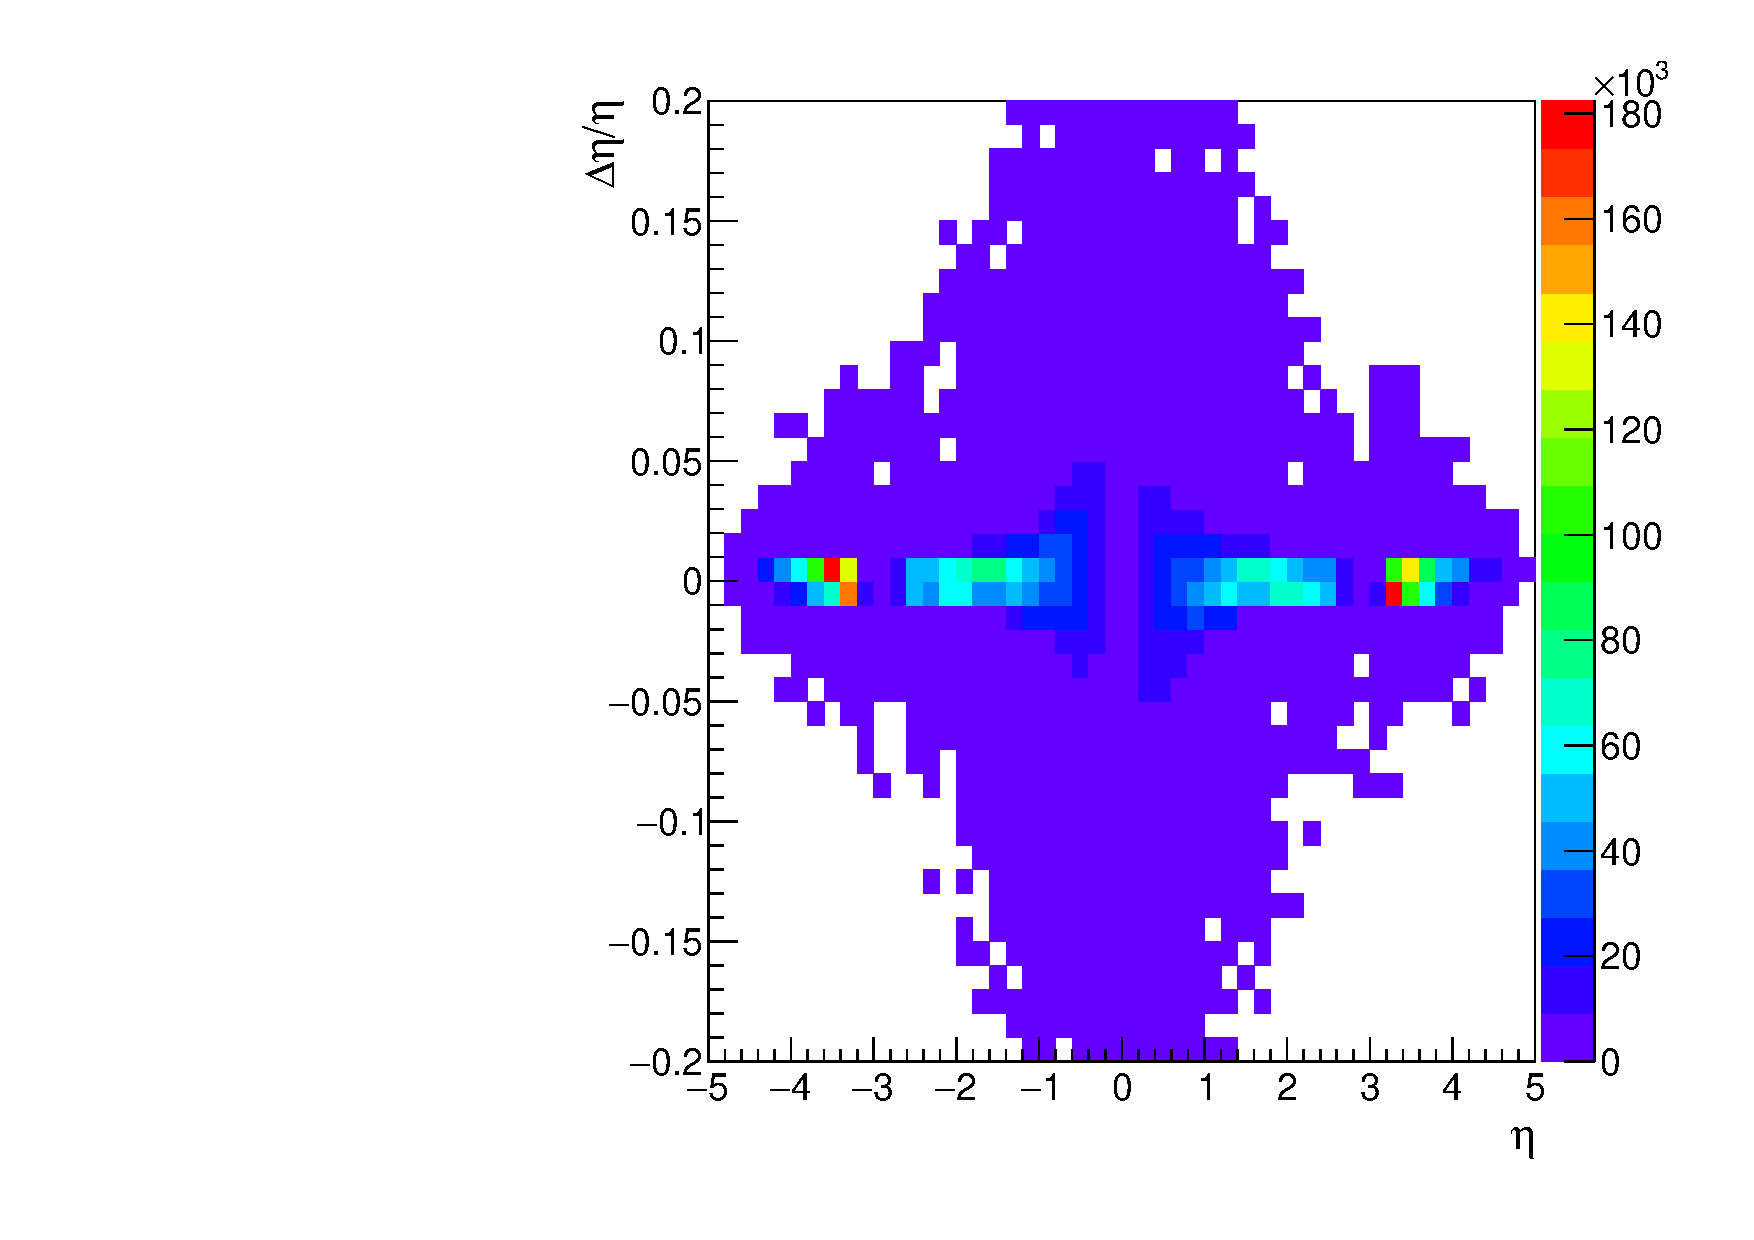
\includegraphics[width=1\linewidth]{Offline_2C_etaRatio_Leading_Non_BJet}
		\end{minipage}
		\caption[\dee for the leading non-\bjet\ in data and Monte-Carlo simulations]{\dee for the leading non-\bjet, for Monte-Carlo simulation in the left panel and data in the right panel.}
		\label{fig:O:leadingnonbeta}
	\end{figure}

	\begin{figure}[h]
		\centering
		\begin{minipage}[h]{0.47\linewidth}
			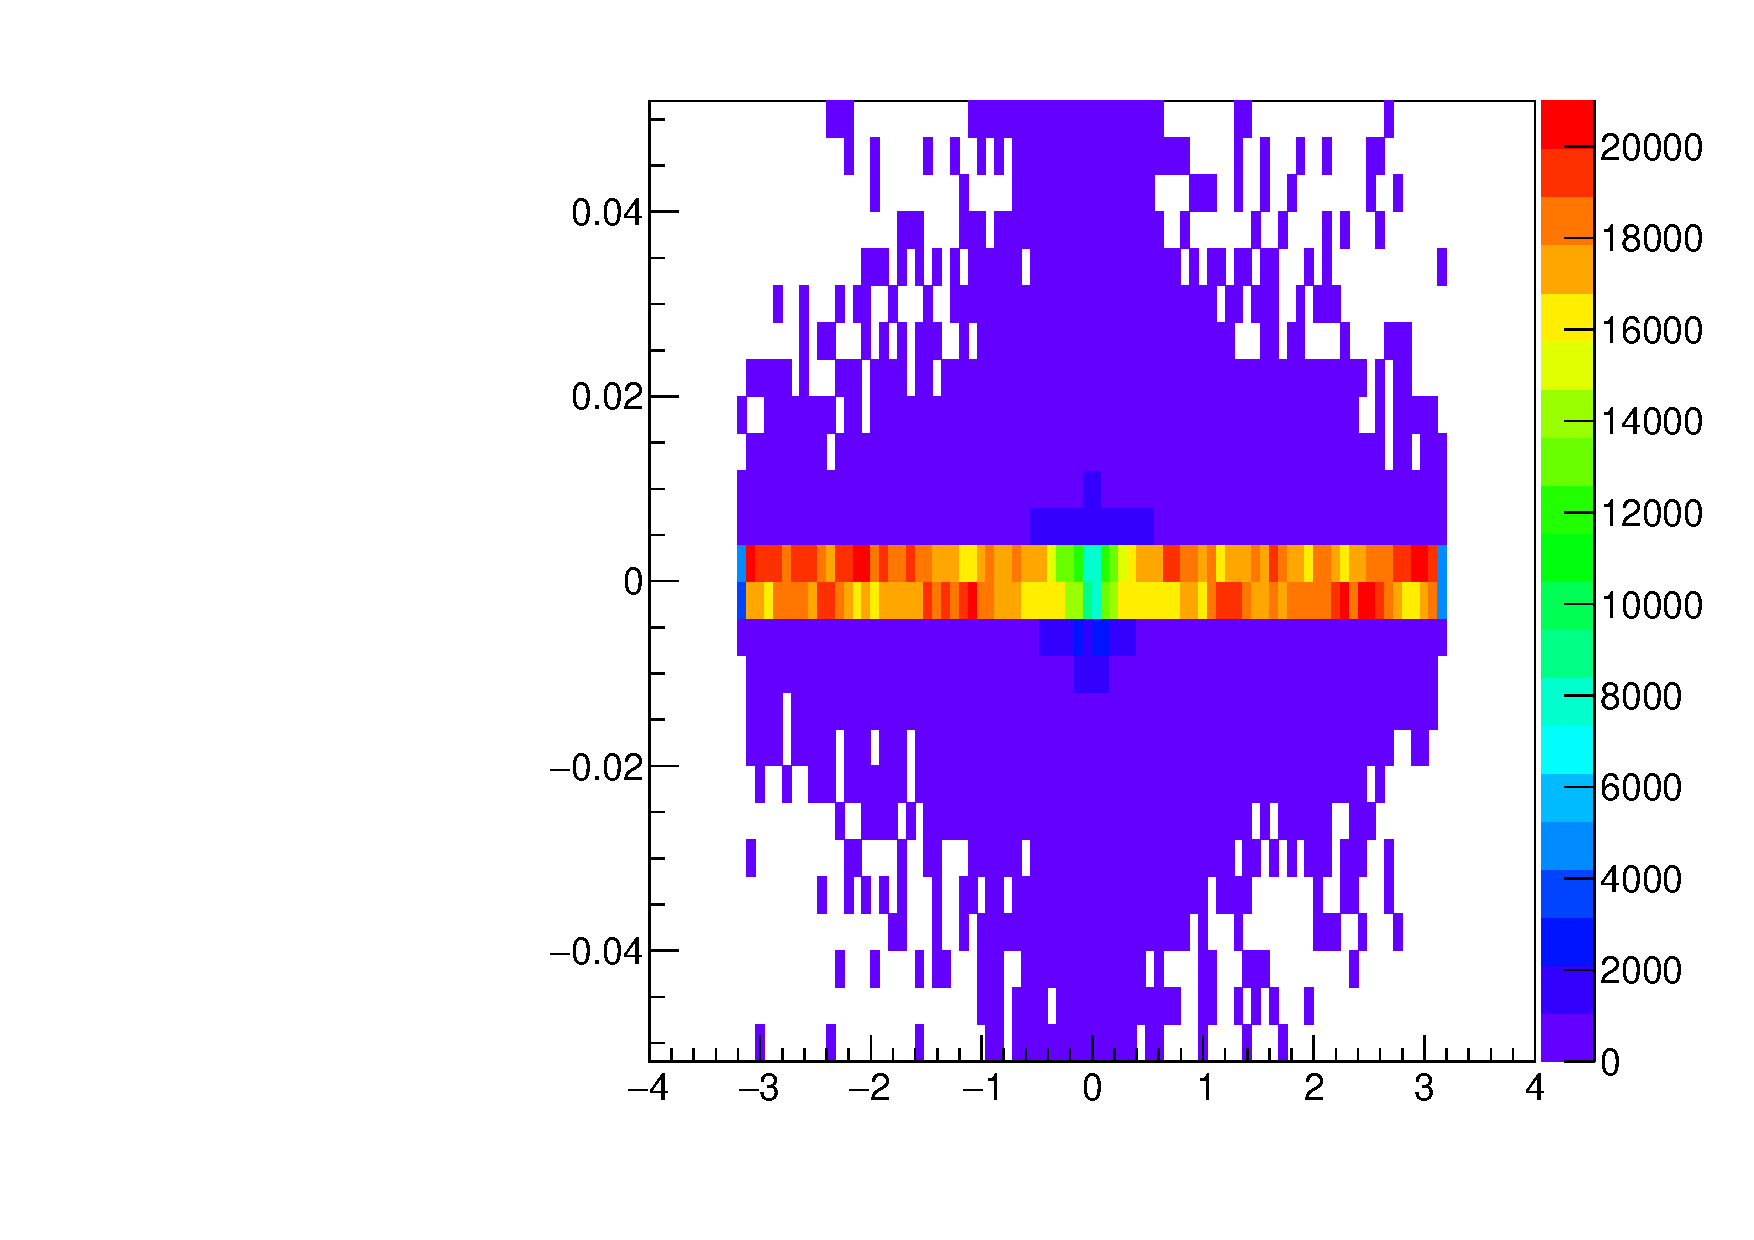
\includegraphics[width=1\linewidth]{phiRatio_Leading_Non_BJet}

		\end{minipage}
		\begin{minipage}[h]{0.47\linewidth}
			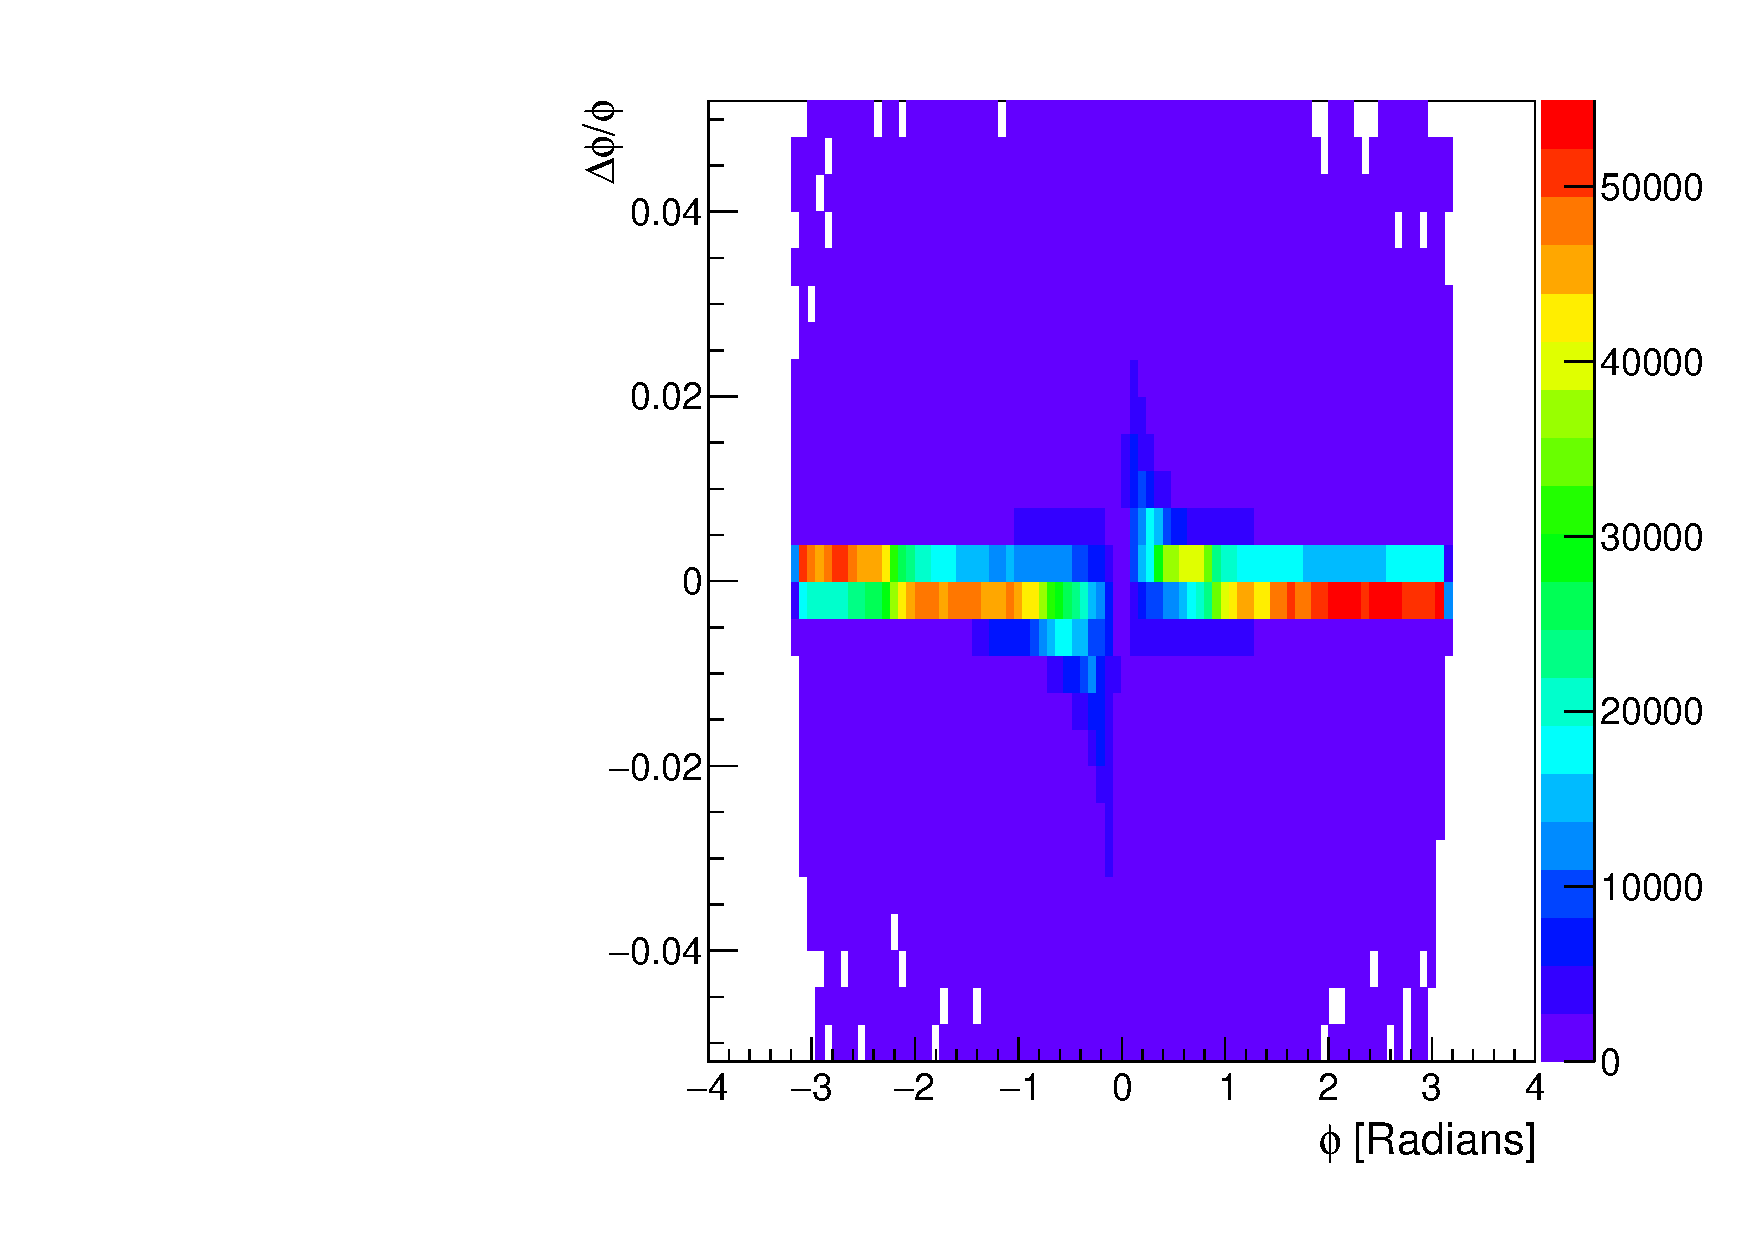
\includegraphics[width=1\linewidth]{Offline_2C_phiRatio_Leading_Non_BJet}
		\end{minipage}
		\caption[\dphph for the leading non-\bjet\ in data and Monte-Carlo simulations]{\dphph for the leading non-\bjet, for Monte-Carlo simulation in the left panel and data in the right panel.}
		\label{fig:O:leadingnonbphi}
	\end{figure}

	These \dxx values can be calculated and plotted for the topological kinematic quantities ($\eta$,~$\phi$), with \dee for the leading non-\bjet\ plotted in Figure \ref{fig:O:leadingnonbeta} against the offline jet $\eta$, and \dphph against offline $\phi$ plotted in Figure \ref{fig:O:leadingnonbphi}. As with the \bjets\, the ($\eta$,~$\phi$) values of the offline and online jets produce nearly identical results, with the distribution of \dxx firmly centred around 0 and a width of less than $1\%$. As with the \bjets, this shows the spatial position of the leading non-\bjet\ is comparable for online and offline objects.


	\subsection{Summary of Comparison of Jet Objects between Offline and Online}
	\label{obp:jetsum}

		The jet objects reconstructed in the HLT have some slight differences in the reported values for key topological variables, but overall they perform in a similar fashion, both in Monte-Carlo simulations and in data. The positional variables $\phi$ and $\eta$ are directly comparable between offline and online jet objects, with the majority of objects having values with $<1\%$ disagreement for both \bjets\ and non-\bjets. For the \pt of jet objects, the values are not in perfect agreement, but have a consistent offset observed in Monte-Carlo simulation and data.

		This difference in jet energy scale calibration can easily be overcome by constructing  or using specific online jet calibrations using already standard jet calibration tools \cite{JES, jetcalib} to correct the offset of the \pt values.

		With this calibration executed on the HLT jet objects, the online jets would then be directly comparable in energy scale and topographical location to the offline jet objects, and as such would be usable in analyses as a replacement for the offline objects. Further verification of this could be carried out by emulating the trigger for the Monte-Carlo simulation to check if the same features arise in the kinematic quantity distributions.

\section{Jet Tagging Efficiency}

	As covered in Section  \ref{det:btag:mv}, the standard algorithm for 2016 physics analyses was chosen to be the 2016 MV2c10 algorithm. However, the HLT \btag\, algorithm uses the older MV2c20 algorithm \cite{trig2015}. For any form of a Trigger Level Analysis to be considered valid, the performance of the tagging algorithms used in the trigger, which are fixed at the point of data collection, must be comparable with the tagging executed offline with more up to date \btag\, configurations.

	To study this, the \btag\, efficiency at trigger level and offline is studied for different jet flavours using the Monte-Carlo sample. The Monte-Carlo sample was used as the \textit{truth} nature of the jet object is known, and the result of the \btag\, algorithm can be compared for \bjets, \cjets\, and light-jets.

	In the analysis, an offline/HLT jet pair was formed using $\Delta R$ matching and using the truth label of the offline jet to assign a flavour to the pair. Light-jets, \bjets\, and \cjets\, were all studied separately to view the \btag\, efficiency and the mistag rate of both algorithms operating at the \textit{tight} working point for an expected \btag\ efficiency of $70\%$. The efficiency plots in Figures \ref{fig:MC:bjetefficiency}, \ref{fig:MC:cjetefficiency} and \ref{fig:MC:lightjetefficiency} show the fraction of these jets that were identified as \bjets\, by the HLT and offline tagging algorithms. These plots were created from events following the same cuts as for the leading \bjet\ and non-\bjet\ as discussed at the beginning of the chapter.

	\subsection{\textit{b}-jet efficiency}
	\label{obp:beff}

	For jets labeled as true \bjets, the tagging efficiency can be calculated and plotted against kinematic quantities of the \bjets. Figure \ref{fig:MC:bjetefficiency} shows the \btag\ efficiency $\epsilon$ plotted against the \pt and $\eta$ of the offline \bjet.

		\begin{figure}[h]
			\centering
			\begin{minipage}[h]{0.48\linewidth}
				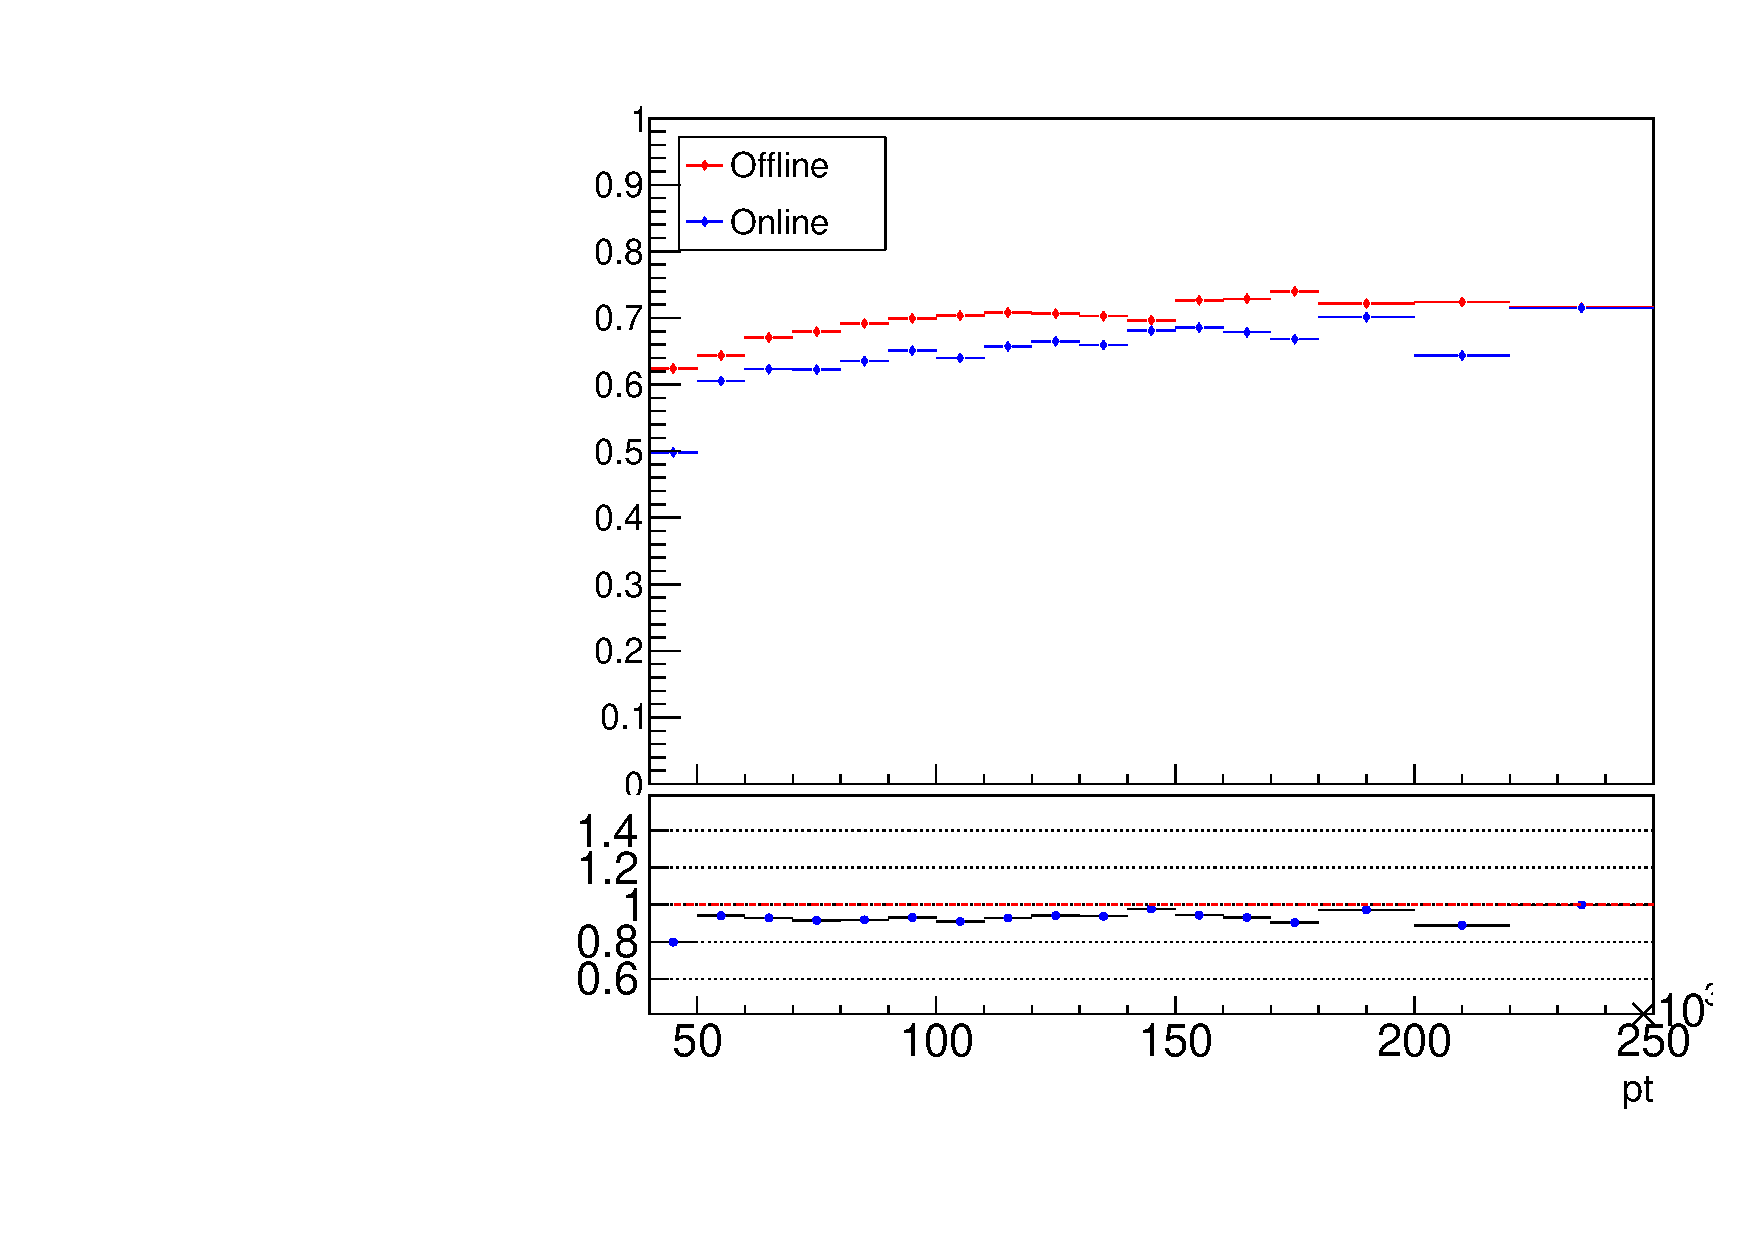
\includegraphics[width=1\linewidth]{ptBJET}

			\end{minipage}
			\quad
			\begin{minipage}[h]{0.48\linewidth}
				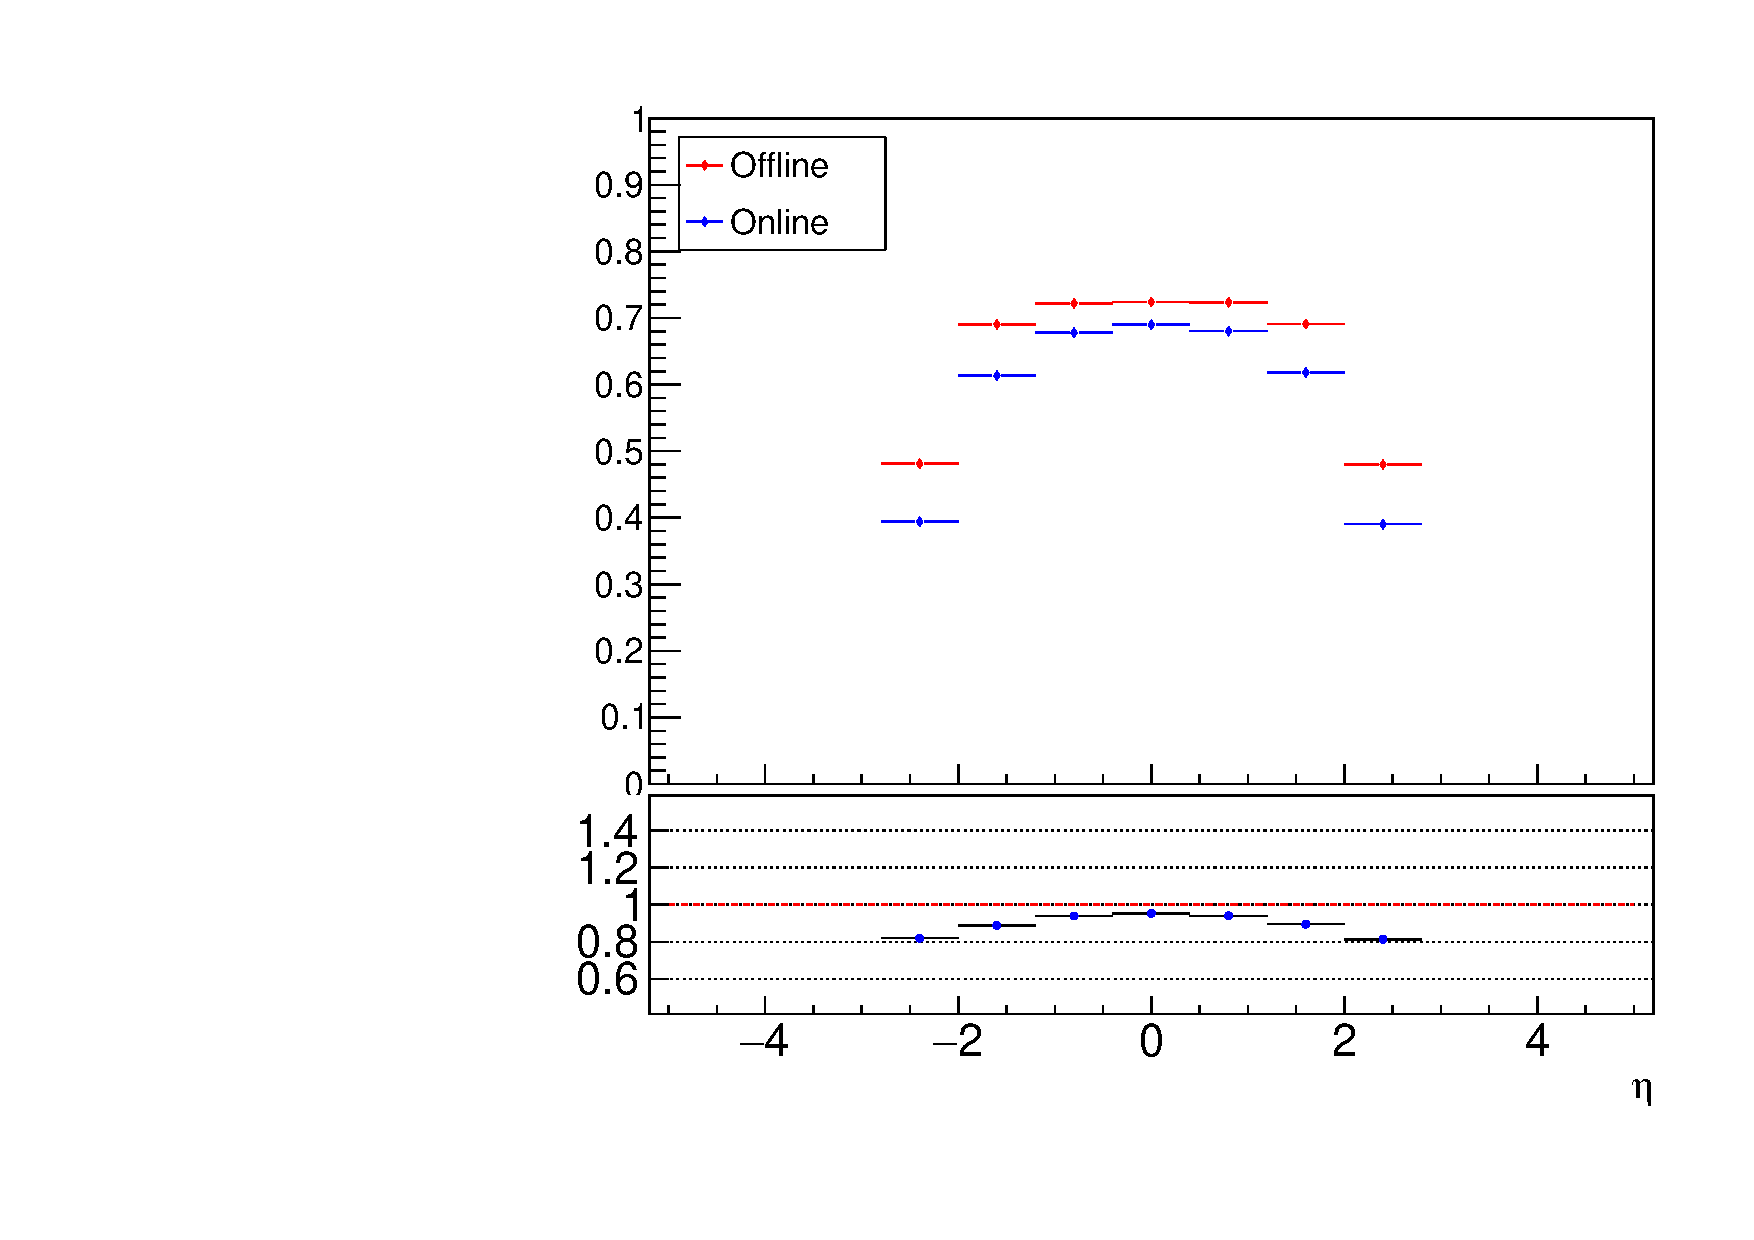
\includegraphics[width=1\linewidth]{etaBJET}
			\end{minipage}
			\caption[Comparison of \bjet\ tagging efficiency on truth \bjets\ between online and offline jets in Monte-Carlo simulation]{\btag\, efficiency for truth \bjets\, in Monte-Carlo simulation, evaluated for offline jets with the 2016 MV2c10 algorithm and for online jets with the 2015 MV2c20 algorithm, plotted against offline jet \pt in the left panel and offline jet $\eta$ in the right panel.}
			\label{fig:MC:bjetefficiency}
		\end{figure}

		The overall distribution shape in \pt and $\eta$ for the \btag\ efficiency is consistent for both the online and offline \bjet. The shape of the distribution in \pt shown in the left panel of Figure \ref{fig:MC:bjetefficiency} is consistent with the efficiency curves expected for the MV2 \btag\ algorithm with respect to \pt \cite{btagOptimisation}, and the efficiency is consistent with the $70\%$ value expected for the \textit{tight} working point for the offline jets, shown clearly by the flat peak of the $\eta$ distribution in the right panel for the central $\eta$ regions.

		However, the HLT \btag\, is shown to be around 5\% less efficient than the offline \btag\, for jets with \pt$>50$GeV. This value is consistent across the \pt distribution shown by the flat line at $\sim0.95$ in the ratio plot in the left panel of Figure \ref{fig:MC:bjetefficiency}. The improvement in efficiency between the 2016 MV2c10 and 2015 MV2c20 algorithms is consistent with the comparative behaviour shown for a training $t\bar{t}$ sample \cite{btagOptimisation}, but of a larger magnitude. The performance will also differ as the computational time available for the online algorithm is greatly reduced compared to the offline tagging. This requires a less precise tracking algorithm which will perform slightly worse than the offline algorithm, which should account for some of the difference.

		This change in efficiency, consistent with the differences in the two algorithms, could be rectified by applying the newer algorithm to the online jet objects. However, the trigger-level jet objects in the xAOD sample data only contained the discriminant values from the applied 2015 MV2c20 algorithm which could be extracted using standard \btag\ tools in AnalysisBase. The input variables used for the training and evaluation of the component algorithms of the MV2 algorithms (Section \ref{det:btagging}) were discarded from the HLT level jet objects. Retaining these quantities on the online jets would allow future trigger-level analyses to make use of the newer \btag\ algorithms or retrain one algorithm to increase the performance to offline levels. This would result in an increased detector readout size in bytes, which could reduce the permitted rate increase for a trigger-object level analysis. An estimate of such a resultant decrease in rate requires further work beyond the scope of this dissertation.

	\subsection{\textit{c}-jet efficiency}
	The same efficiency plot could be produced for \cjets\, against the kinematic jet quantities. Any result marked as a \bjet\ for a truth \cjet\ is a mistagged jet, and plots of the efficiency show measurements of the mistag rate of the algorithm. The mistag rate is plotted in Figure \ref{fig:MC:cjetefficiency} for the online and offline jets against offline \pt and $\eta$.
		\begin{figure}[h]
			\centering
			\begin{minipage}[h]{0.48\linewidth}
				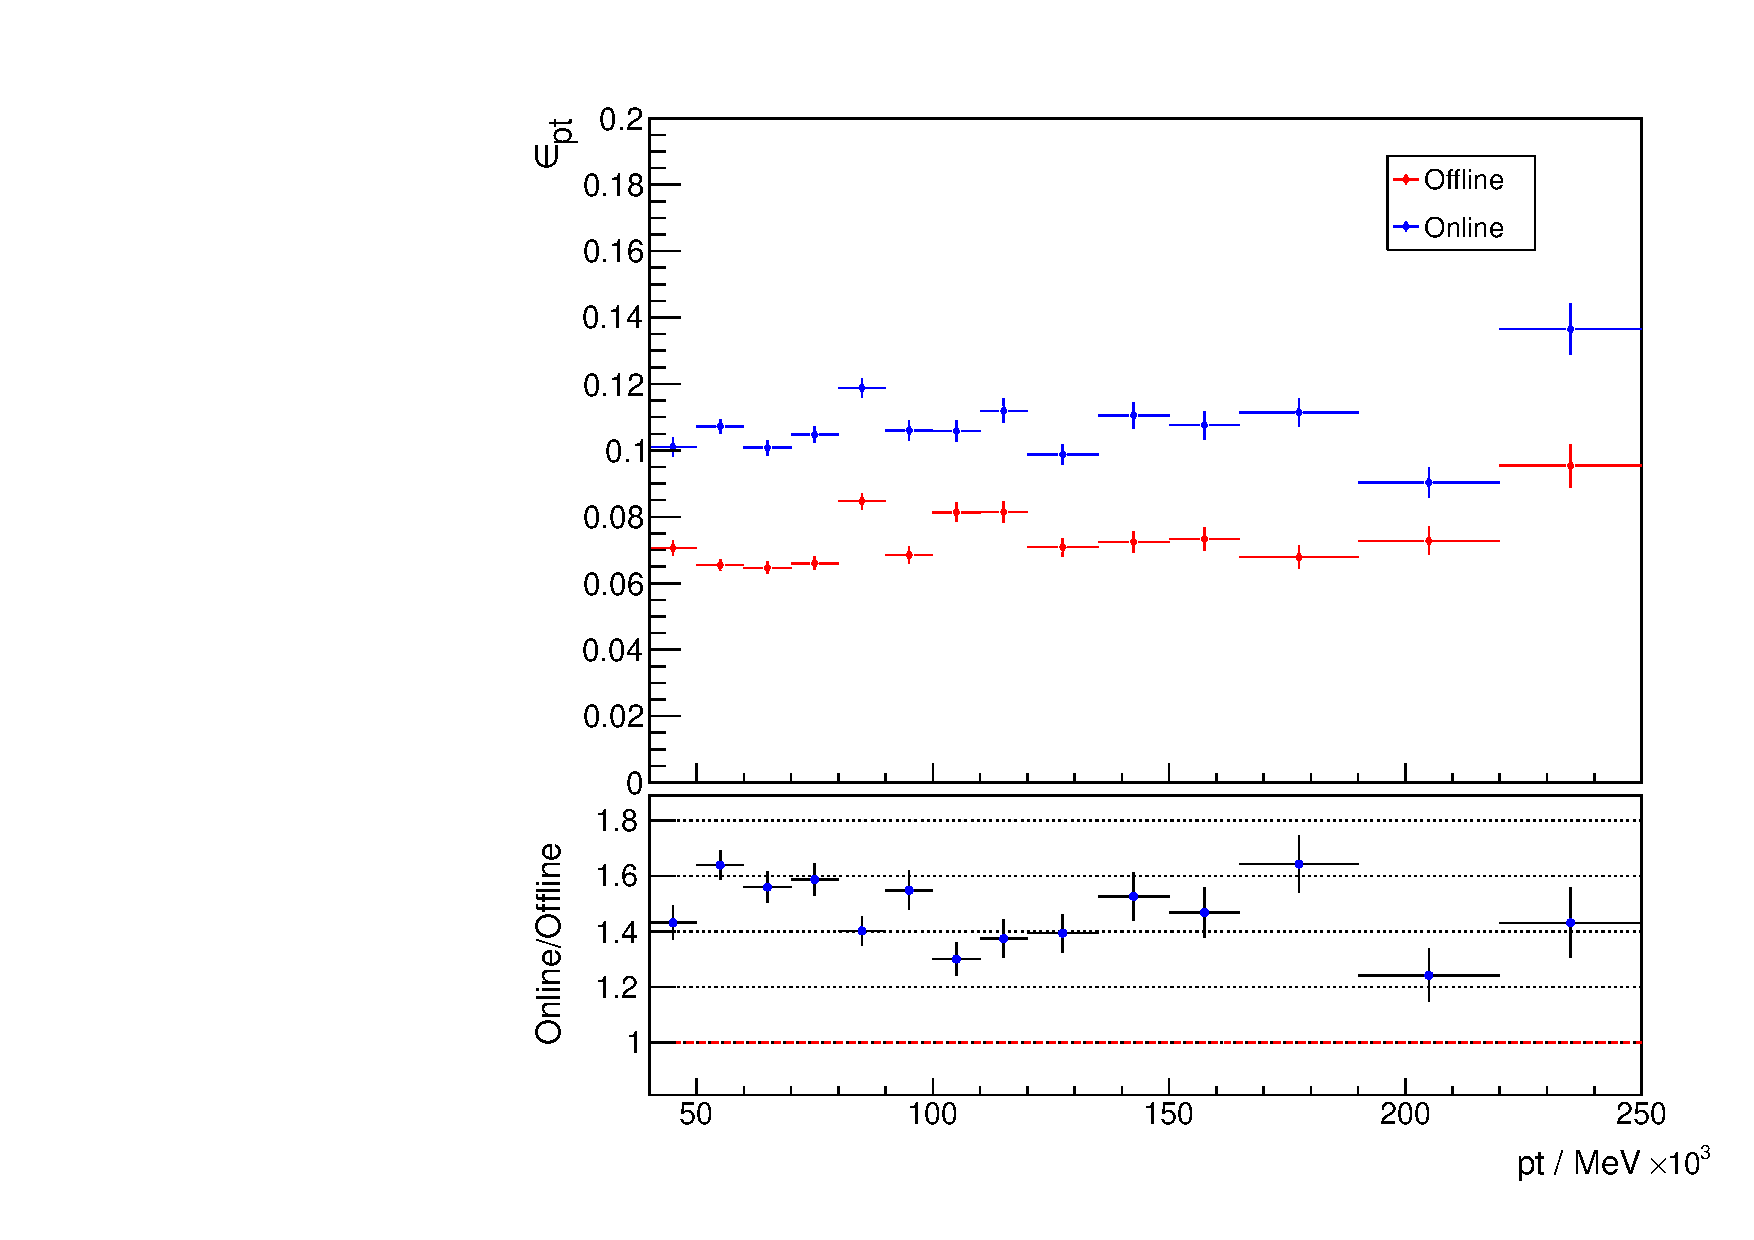
\includegraphics[width=1\linewidth]{ptCJET}

			\end{minipage}
			\quad
			\begin{minipage}[h]{0.48\linewidth}
				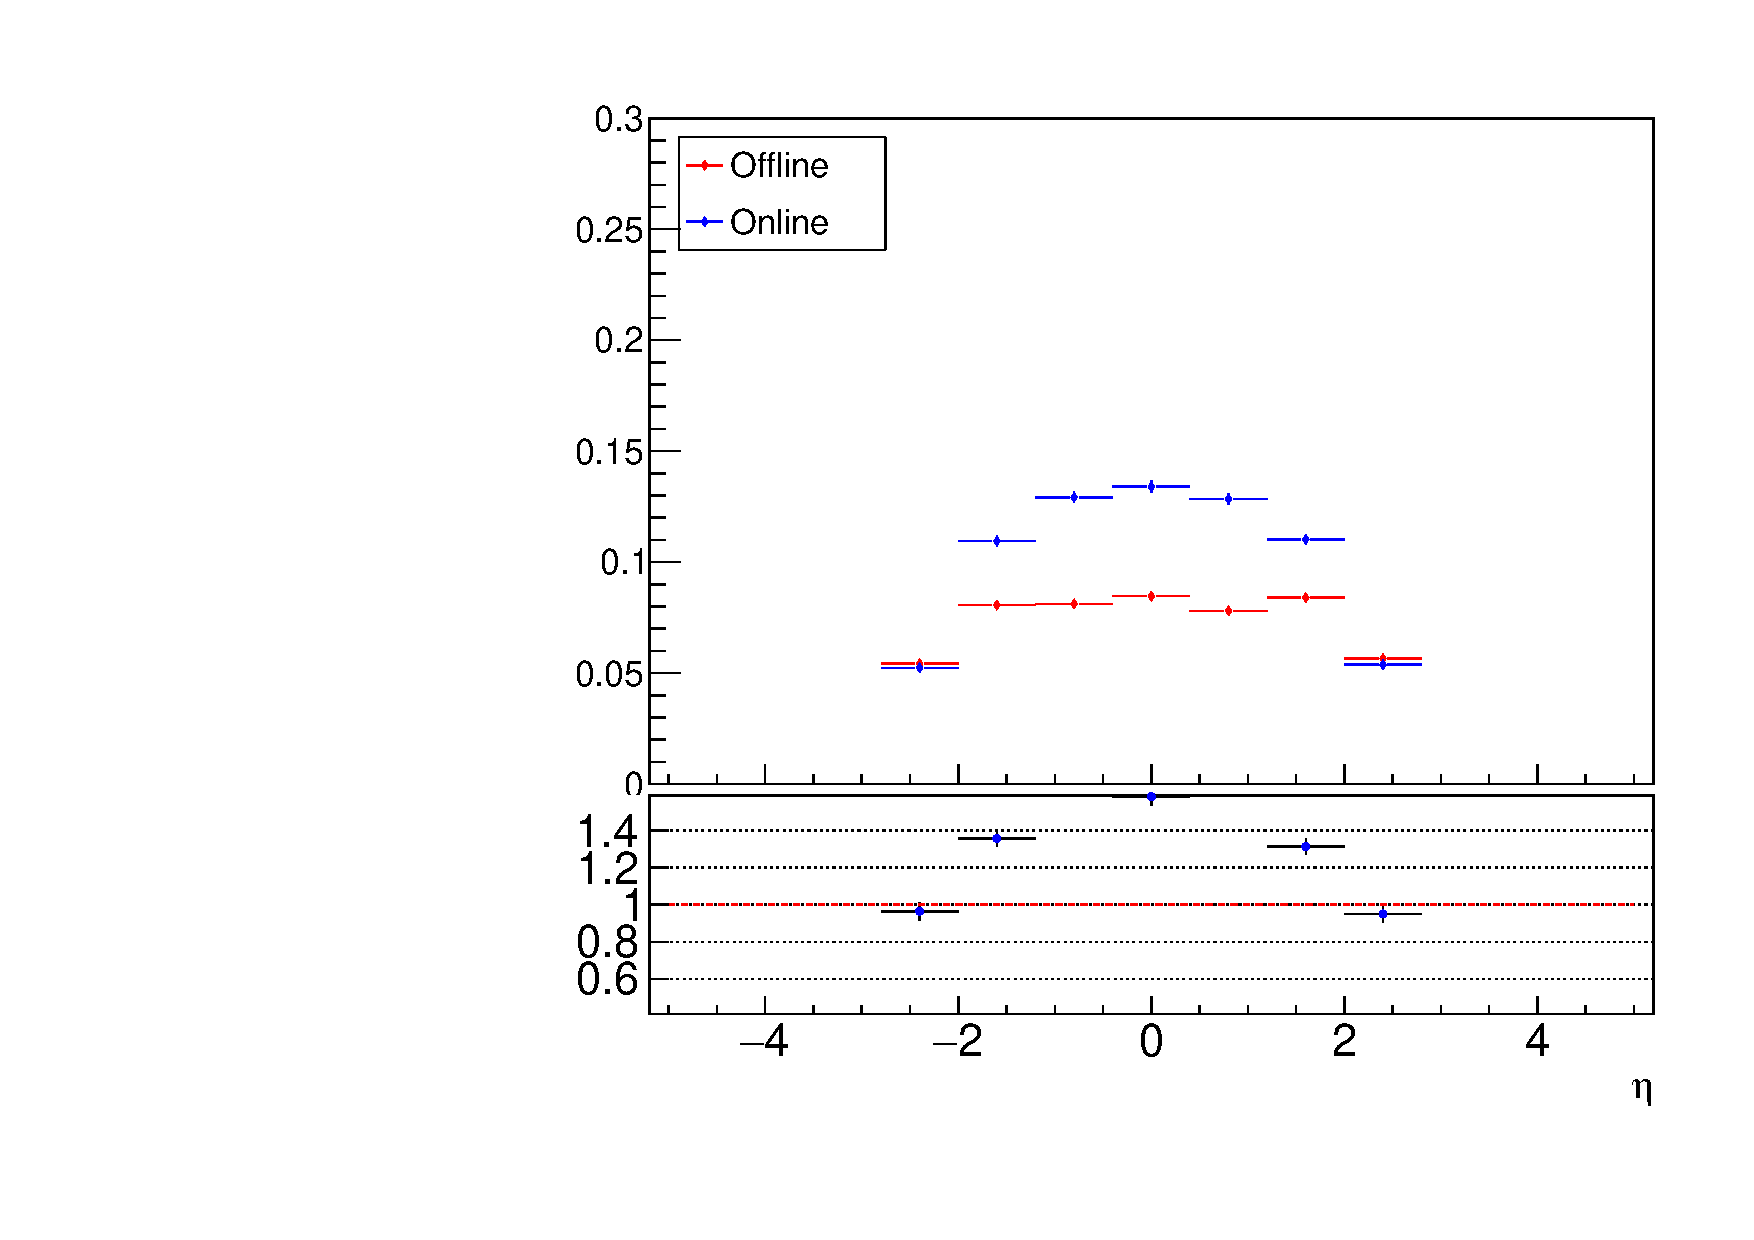
\includegraphics[width=1\linewidth]{etaCJET}
			\end{minipage}
			\caption[Comparison of mistag rate between online and offline truth \cjets\ in Monte-Carlo simulation]{Mistag rate for truth \cjets\, in Monte-Carlo simulation, evaluated for offline jets with the 2016 MV2c10 algorithm and for online jets with the 2015 MV2c20 algorithm, plotted against offline jet \pt in the left panel and offline jet $\eta$ in the right panel.}
			\label{fig:MC:cjetefficiency}
		\end{figure}

		The shape of the mistag rate distribution is more noisy than the \bjet\ efficiency plots in Figure \ref{fig:MC:bjetefficiency}, but across the \pt distribution in the left panel of Figure \ref{fig:MC:cjetefficiency} the online mistag rate is $\sim50\%$ higher than the offline rate.

		The increase in the rate of \cjet\, mistagging is absolutely consistent with the refinements to the algorithm between the 2016 MV2c10 and 2015 MV2c20, with increased levels of \cjet\, rejection in the offline 2016 MV2c10, and the increase is consistent with the expected shift from the optimised algorithm \cite{btagOptimisation}. Similar to the solution for changes in \btag\ efficiency in Section \ref{obp:beff}, retaining the inputs to the \btag\ algorithms would allow improved versions of the \btag\ algorithms to be applied to the HLT jets.

	\subsection{Light-jet efficiency}

		Plots of the mistag rate for truth light-jets for online and offline \btag\ against the offline jet \pt and $\eta$ are shown in Figure \ref{fig:MC:lightjetefficiency}

		\begin{figure}[h]
			\centering
			\begin{minipage}[h]{0.48\linewidth}
				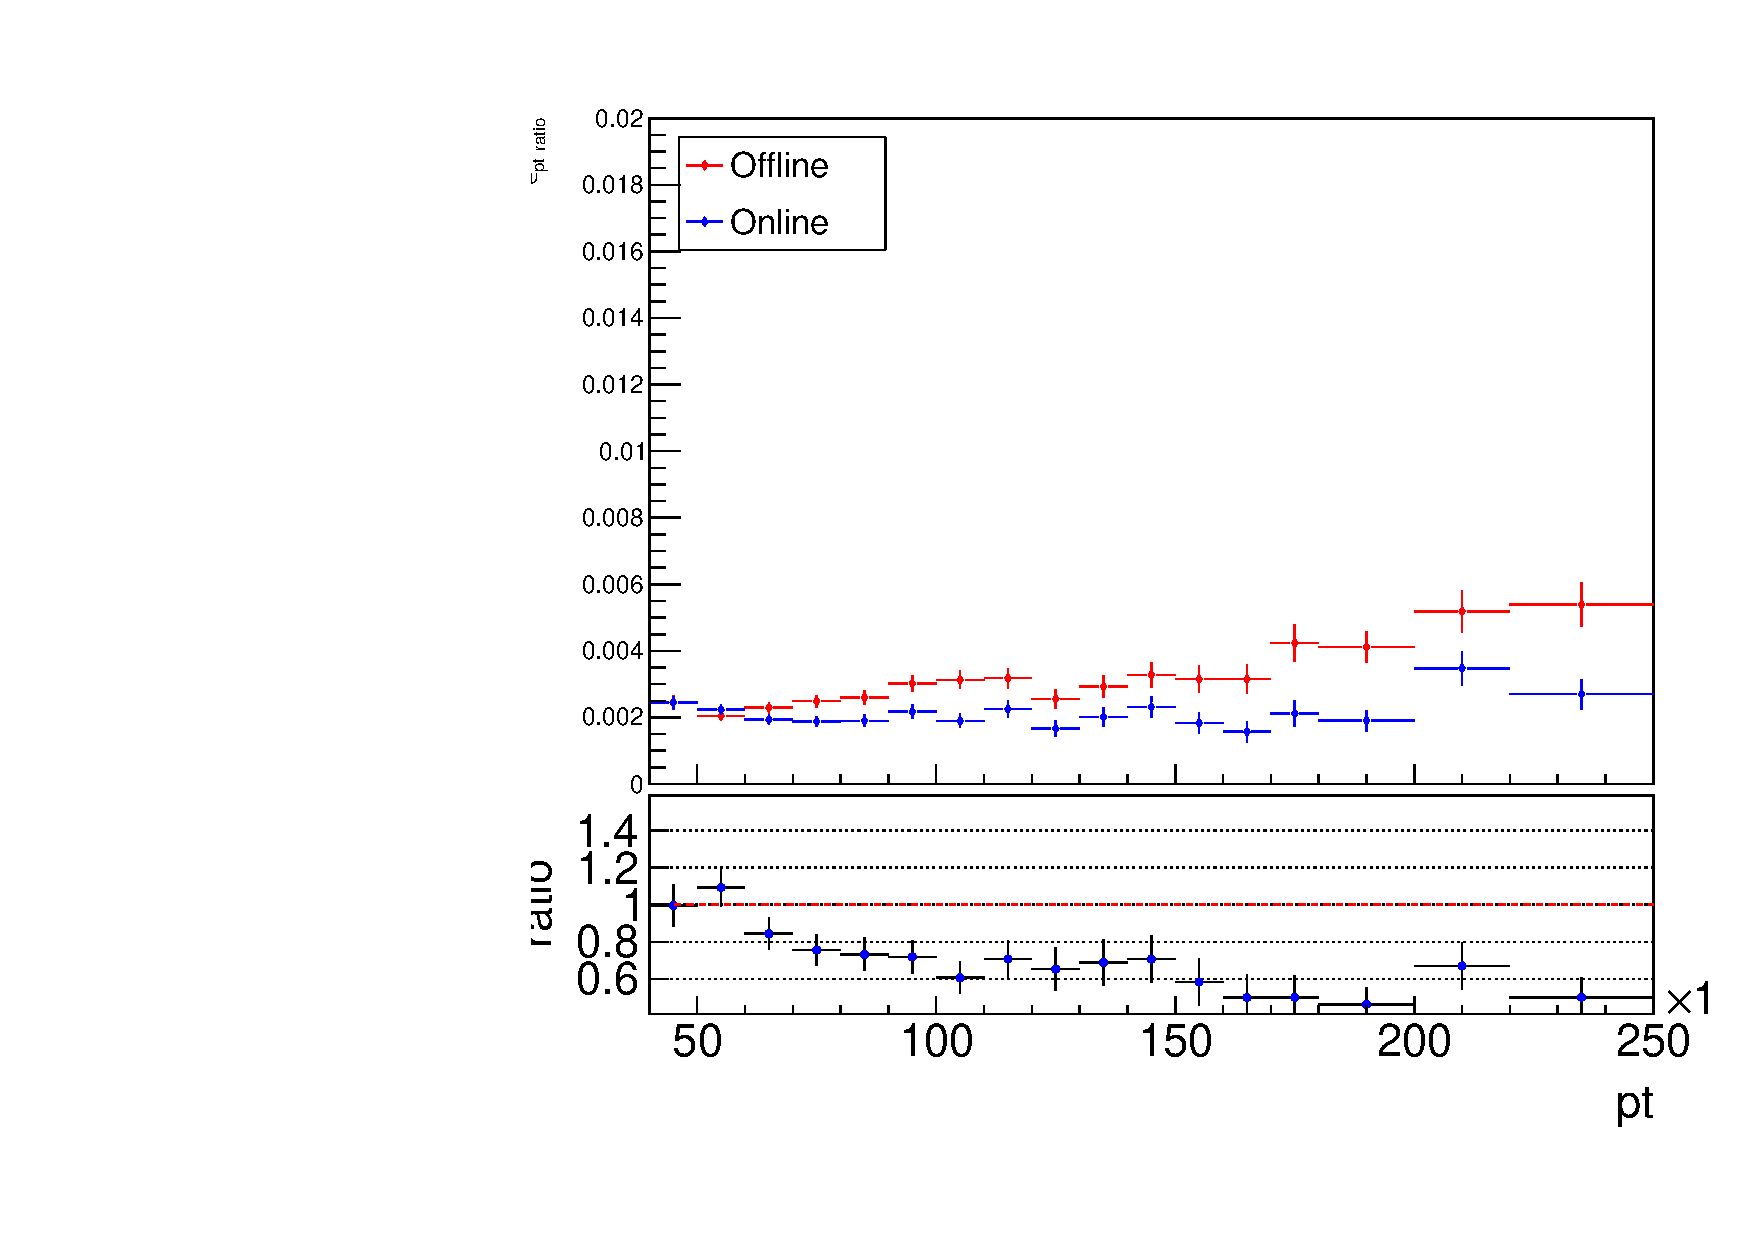
\includegraphics[width=1\linewidth]{ptLIGHTJET}

			\end{minipage}
			\quad
			\begin{minipage}[h]{0.48\linewidth}
				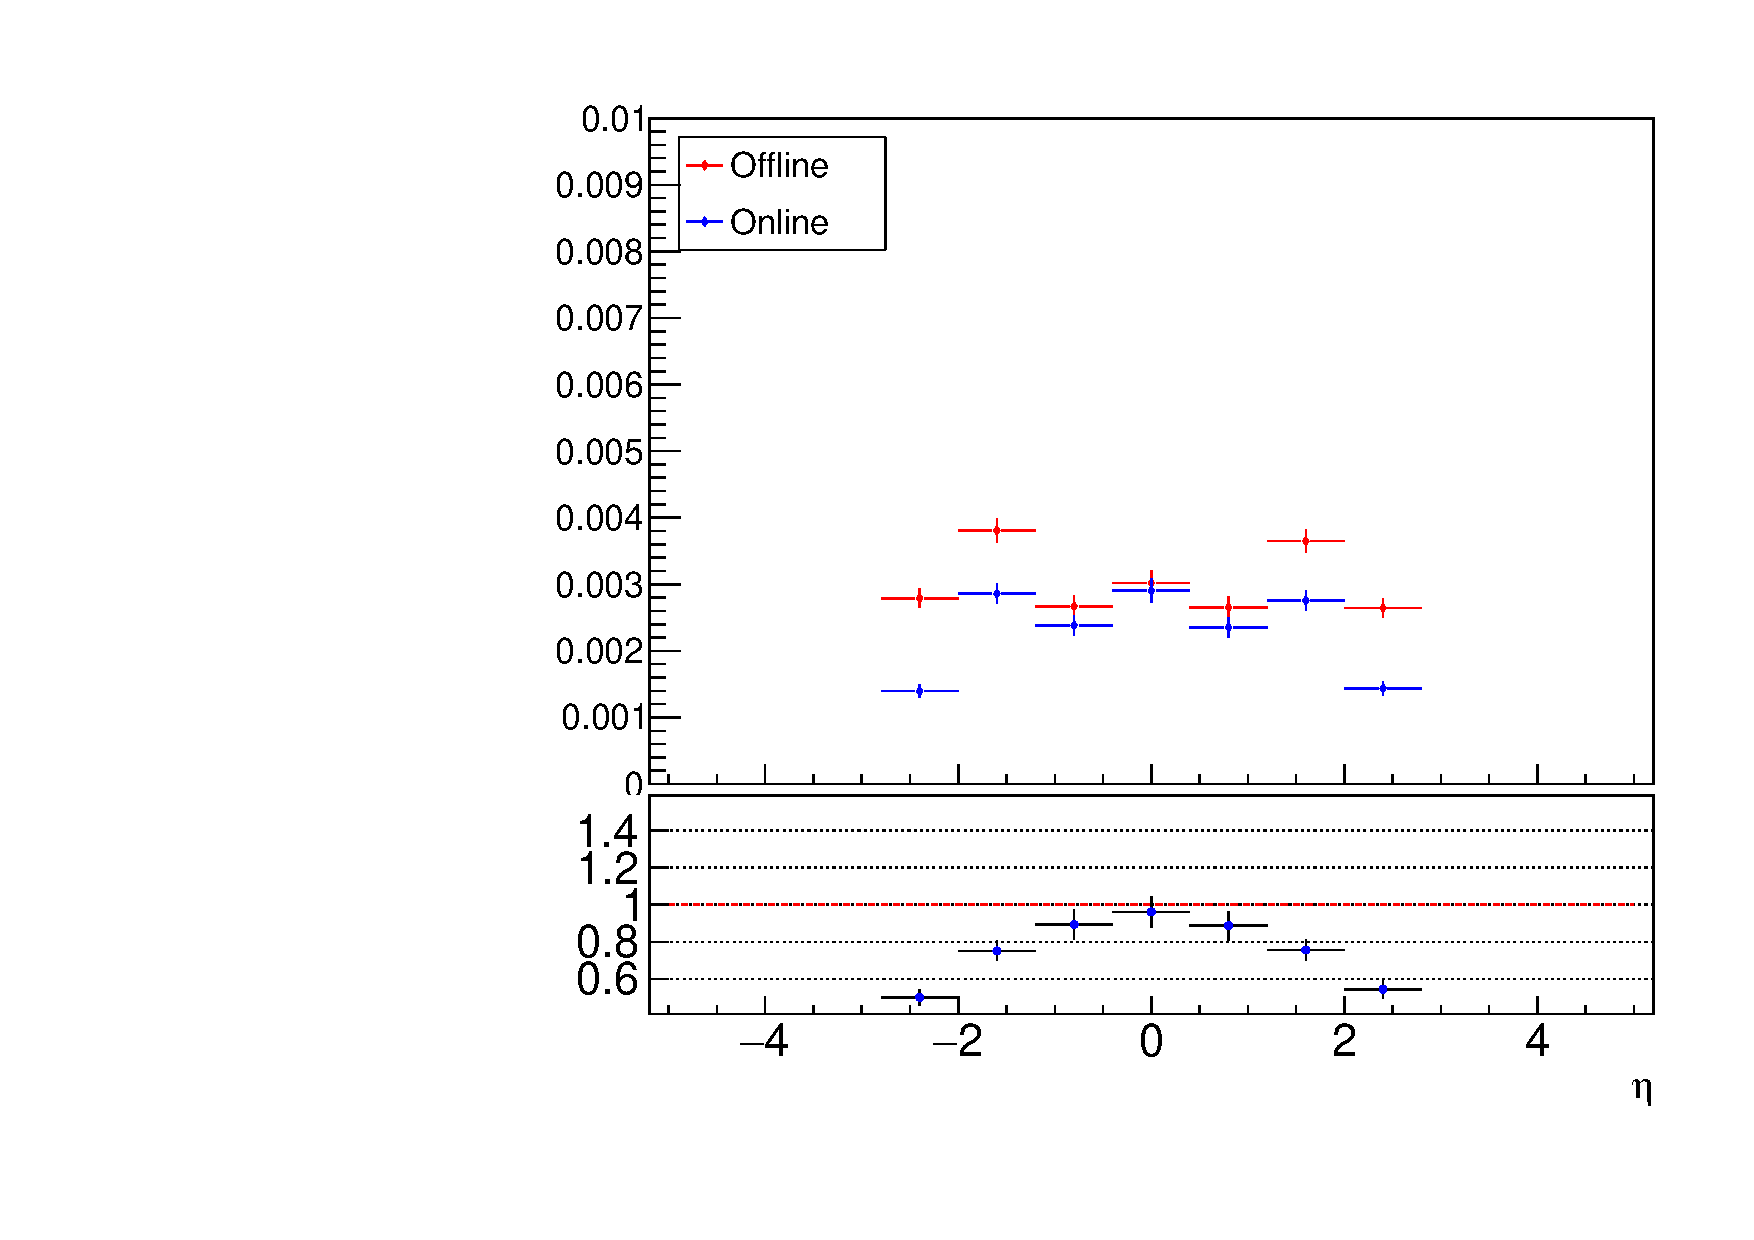
\includegraphics[width=1\linewidth]{etaLIGHTJET}
			\end{minipage}
			\caption[Comparison of mistag rate between online and offline truth light-jets in Monte-Carlo simulation]{Mistag rate for truth light-jets in Monte-Carlo simulation, evaluated for offline jets with the 2016 MV2c10 algorithm and for online jets with the 2015 MV2c20 algorithm, plotted against offline jet \pt in the left panel and offline jet $\eta$ in the right panel}
			\label{fig:MC:lightjetefficiency}
		\end{figure}

		The light-jet efficiency plots are noisier than the plots for truth \bjets\ and \cjets\ owing to the low mistag rate of $\sim0.3\%$, as shown in the left panel of Figure \ref{fig:MC:lightjetefficiency}. For these light-jets, the online algorithm performs better than the offline algorithm overall, with a mistag rate of equal to $\sim80\%$ the offline rate for jets with \pt$<150$. The change in the performance for the light-jet rejection, with the 2015 MV2c20 algorithm performing better for higher \pt values and worse for lower \pt values, is consistent with the expected change in behaviour between the two algorithms \cite{btagOptimisation}.


	\subsection{Tag Matching}

	For each pair of jets that could be matched between online and offline, and then successfully have a \btag\, decision evaluated on the jets, the agreement of the \btag\, between the two jets was checked. These were found to match one another in $91\%$ of cases.

	\section{Summary}

	The aim of this section of the analysis was to show that using online reconstructions of the constituent jet objects used in a \VBFHBB\ analysis was comparable to using offline objects by showing the properties of the jets and the \btag\ of the jets to be similar. The overall performance using the HLT objects as constructed during the data-taking and in the Monte-Carlo simulations is similar to the offline behaviour. The topological jet quantities ($\eta$, $\phi$) are directly comparable between the two types of jet objects. However there are differences between the \pt values of the HLT and offline jet objects and differences between the performances of the \btag\ algorithms.

	These differences are readily rectifiable however. The energy scale calibration differences can be accounted for using standard jet calibration tools to bring the \pt values of the online and offline jets into agreement with one another \cite{JES}, while the \btag\ performance can be made similar if the input variables to the MV2 algorithm are preserved on the trigger-level jet object, such that more developed \btag\ algorithms can be applied to the jet instead of the algorithm used during data collection.

	With these corrections, there are no differences between the trigger level objects making up a \VBFHBB\ event and the offline objects that would prohibit a TLA analysis of the \VBFHBB\ channel.

\endinput
